%definira klasu dokumenta 
\documentclass[12pt]{report} 

%prostor izmedu naredbi \documentclass i \begin{document} se zove uvod. U njemu se nalaze naredbe koje se odnose na cijeli dokument
	
	%osnovni LaTex ne može riješiti sve probleme, pa se koriste različiti paketi koji olakšavaju izradu željenog dokumenta
	\usepackage[croatian]{babel} 
	\usepackage{amssymb}
	\usepackage{amsmath}
	\usepackage{txfonts}
	\usepackage{mathdots}
	\usepackage{titlesec}
	\usepackage{array}
	\usepackage{lastpage}
	\usepackage{etoolbox}
	\usepackage{tabularray}
	\usepackage{color, colortbl}
	\usepackage{adjustbox}
	\usepackage{geometry}
	\usepackage[classicReIm]{kpfonts}
	\usepackage{hyperref}
	\usepackage{fancyhdr}
	\usepackage{graphicx}
        \usepackage{subcaption}
	\graphicspath{ {./img/} }
	
	\usepackage{float}
	\usepackage{setspace}
	\restylefloat{table}

        % -- Loading the code block package:
        \usepackage{listings}
        % -- Defining colors:
        \usepackage[dvipsnames]{xcolor}
        \definecolor{codegreen}{rgb}{0,0.6,0}
        \definecolor{codegray}{rgb}{0.5,0.5,0.5}
        \definecolor{codepurple}{rgb}{0.58,0,0.82}
        \definecolor{backcolour}{rgb}{0.95,0.95,0.92}
        % Definig a custom style:
        \lstdefinestyle{mystyle}{
            backgroundcolor=\color{backcolour},   
            commentstyle=\color{codepurple},
            keywordstyle=\color{NavyBlue},
            numberstyle=\tiny\color{codegray},
            stringstyle=\color{codepurple},
            basicstyle=\ttfamily\footnotesize\bfseries,
            breakatwhitespace=false,         
            breaklines=true,                 
            captionpos=t,                    
            keepspaces=true,                 
            numbers=left,                    
            numbersep=5pt,                  
            showspaces=false,                
            showstringspaces=false,
            showtabs=false,                  
            tabsize=2
        }

        \lstset{style=mystyle}
	
	
	\patchcmd{\chapter}{\thispagestyle{plain}}{\thispagestyle{fancy}}{}{} %redefiniranje stila stranice u paketu fancyhdr
	
	%oblik naslova poglavlja
	\titleformat{\chapter}{\normalfont\huge\bfseries}{\thechapter.}{20pt}{\Huge}
	\titlespacing{\chapter}{0pt}{0pt}{40pt}
	
	
	\linespread{1.3} %razmak između redaka
	
	\geometry{a4paper, left=1in, top=1in,}  %oblik stranice
	
	\hypersetup{ colorlinks, citecolor=black, filecolor=black, linkcolor=black,	urlcolor=black }   %izgled poveznice
	
	
	%prored smanjen između redaka u nabrajanjima i popisima
	\newenvironment{packed_enum}{
		\begin{enumerate}
			\setlength{\itemsep}{0pt}
			\setlength{\parskip}{0pt}
			\setlength{\parsep}{0pt}
		}{\end{enumerate}}
	
	\newenvironment{packed_item}{
		\begin{itemize}
			\setlength{\itemsep}{0pt}
			\setlength{\parskip}{0pt}
			\setlength{\parsep}{0pt}
		}{\end{itemize}}
	
	%boja za privatni i udaljeni kljuc u tablicama
	\definecolor{LightBlue}{rgb}{0.9,0.9,1}
	\definecolor{LightGreen}{rgb}{0.9,1,0.9}
	
	%Promjena teksta za dugačke tablice
	\DefTblrTemplate{contfoot-text}{normal}{Nastavljeno na idućoj stranici}
	\SetTblrTemplate{contfoot-text}{normal}
	\DefTblrTemplate{conthead-text}{normal}{(Nastavljeno)}
	\SetTblrTemplate{conthead-text}{normal}
	\DefTblrTemplate{middlehead,lasthead}{normal}{Nastavljeno od prethodne stranice}
	\SetTblrTemplate{middlehead,lasthead}{normal}
	
	%podesavanje zaglavlja i podnožja
	
	\pagestyle{fancy}
	\lhead{Programsko inženjerstvo}
	\rhead{Dog Friendly}
	\lfoot{e404TeamNotFound}
	\cfoot{stranica \thepage/\pageref{LastPage}}
	\rfoot{\today}
	\renewcommand{\headrulewidth}{0.2pt}
	\renewcommand{\footrulewidth}{0.2pt}
	
	\begin{document} 
		
		\begin{titlepage}
			\begin{center}
				\vspace*{\stretch{1.0}} %u kombinaciji s ostalim \vspace naredbama definira razmak između redaka teksta
				\LARGE Programsko inženjerstvo\\
				\large Ak. god. 2022./2023.\\
				
				\vspace*{\stretch{3.0}}
				
				\huge DogFriendly\\
				\Large Dokumentacija, Rev. \textit{2}\\
				
				\vspace*{\stretch{12.0}}
				\normalsize
				Grupa: \textit{e404TeamNotFound}\\
				Voditelj: \textit{Leon  Stjepan Uroić}\\
				
				
				\vspace*{\stretch{1.0}}
				Datum predaje: \textit{13.01.2023.}\\
				
				\vspace*{\stretch{4.0}}
				
				Nastavnik: \textit{Laura Majer}\\
				
			\end{center}
			
		\end{titlepage}
		
		\tableofcontents
		\chapter{Dnevnik promjena dokumentacije}

	\begin{longtblr}[
		label=none
		]{
			width = \textwidth, 
			colspec={|X[2]|X[13]|X[4]|X[3]|}, 
			rowhead = 1
		}
		\hline
		\textbf{Rev.}	& \textbf{Opis promjene/dodatka} & \textbf{Autori} & \textbf{Datum}\\[3pt] \hline
		0.1 & Napravljen predložak dokumentacije.	& Luka \newline Marković & 26.10.2022 		\\[3pt] \hline 
		0.2 & Dodani dionici i funkcionalni zahtjevi.	& Nela \newline Štubelj & 28.10.2022 		\\[3pt] \hline 
		0.3 & Dodan opis projektnog zadatka.	& Filip \newline Jakovina & 29.10.2022 		\\[3pt] \hline
		0.4 & Dodani obrasci uporabe i UML dijagrami.	& Mario Hošnjak,\newline Zoa Horvat & 31.10.2022 		\\[3pt] \hline
        0.5.1 & Arhitektura sustava & David Winkler & 3.11.2022.     \\[3pt] \hline
        0.5.2 & Arhitektura baze podataka & Leon Stjepan Uroić & 2.11.2022    \\[3pt] \hline
        0.6.1 & Ažuriran opis & Luka \newline Marković & 3.11.2022.     
        \\[3pt] \hline
        0.6.2 & Izmjenjen UML i UC & Mario Hošnjak,\newline Zoa Horvat & 3.11.2022.     \\[3pt] \hline
        0.6.3 & Ažurirana arhitektura sustava & David Winkler & 4.11.2022.     \\[3pt] \hline
         0.7 & Dizajn korisničkog sučelja početne stranice i stranice za prijavu korisnika & Nela Štubelj & 6.11.2022.     \\[3pt] \hline
         0.8 & Ažurirana dokumentacija baze podataka & Leon Stjepan Uroić & 7.11.2022.     \\[3pt] \hline
		 0.9 & Dodani sekvencijski dijagrami i ostali zahtjevi & Mario Hošnjak & 10.11.2022.     \\[3pt] \hline
		 0.10 & Napravljeni dijagrami razreda & Filip jakovina & 16.11.2022.     \\[3pt] \hline
		 0.11 & Korekcije i priprema prve verzije dokumentacije & Luka \newline Marković & 18.11.2022.     \\[3pt] \hline
		 \textbf{1.0} & Verzija samo s bitnim dijelovima za 1. ciklus & Svi & 17.11.2022. \\[3pt] \hline 
         1.1 & Upute za puštanje u pogon & Leon Stjepan Uroić & 05.01.2023.     \\[3pt] \hline
         1.2 & Dodan dijagram stanja & Luka \newline Marković & 10.01.2023.     \\[3pt] \hline
         1.3 & Dodan dijagram komponenti & Luka \newline Marković & 10.01.2023.     \\[3pt] \hline
         1.3 & Dodani korištene tehnologije i alati & Luka \newline Marković & 10.01.2023.     \\[3pt] \hline
         1.4 & Dodan dijagram aktivnosti & Nela \newline Štubelj & 11.01.2023.     \\[3pt] \hline
         1.5 & Dodan konceptualni dijagram razreda & Filip Jakovina & 12.01.2023.     \\[3pt] \hline
         1.6 & Dodan dijagram razmještaja & Filip Jakovina & 13.01.2023.     \\[3pt] \hline
         1.7 & Dodano ispitivanje sustava & Mario Hošnjak & 13.01.2023.     \\[3pt] \hline
         1.8 & Dodano ispitivanje komponenti & Luka \newline Marković, Filip Jakovina & 13.01.2023.     \\[3pt] \hline
         \textbf{2.0} & Završna verzija dokumentacije & Svi & 13.01.2023.     \\[3pt] \hline
	\end{longtblr}

		\chapter{Opis projektnog zadatka}

    \section{Cilj i opis zadatka}
    Cilj ovog projekta je razviti programsku podršku za web aplikaciju "Dog Friendly" koja će omogućiti korisnicima da na interaktivnoj karti pronađu prikladne lokacije za druženje sa svojim ljubimcima i time im olakšati kretanje. U svrhu financiranja aplikacije, omogućit ćemo vlasnicima obrta koja su povezana sa psima da postave svoju reklamu na stranicu uz određenu pretplatu.
    
    \section{Problematika zadatka}
    Aplikacija Dog Friendly omogućuje svojim korisnicima kretanje po interaktivnoj karti, ručni unos tržene adrese te, uz dozvolu, lociranje vlastitog uređaja. Korisnici pristupaju aplikaciji preko web stranice gdje se mogu prijaviti kao osnovni korisnik ili vlasnik obrta. Odabirom vrste korisnika im se otvara tražena registracijska forma.
    \newline 
    Za stvaranje računa osnovnog korisnika potrebno je:
        \begin{itemize}
            \item \textbf{ime}
            \item \textbf{prezime}
			\item \textbf{korisničko ime} 
			\item \textbf{e-mail} 
			\item \textbf{lozinku}
			\item \textbf{opis}
		\end{itemize}
    Registriranim korisnicima je osim osnovnih funkcija omogućeno postavljanje novih lokacija, označavanje lokacija prikladnim/neprikladnim za pse, ostavljanje recenzija i komentara na lokacije. 
    \eject
    Za vlasnike obrta je dodatno potrebno unijeti:
    \begin{itemize}
		\item \textbf{ime obrta} 
		\item \textbf{OIB} 
		\item \textbf{e-mail}
		\item \textbf{lozinka}
		\item \textbf{broj telefona}
		\item \textbf{opis}
		\item \textbf{tip obrta}
		\item \textbf{broj kartice}
		\item \textbf{CVV}
		\item \textbf{datum isteka kartice}
	\end{itemize}
	Vlasnici obrta nakon registracije na karti odabiru adrese svojih obrta i postavljaju na njih markere. Prilikom odabira lokacije osnovnom korisniku se prikazuje adresa i javni dio podataka unesen prilikom registracije (ime obrta, kontakt i opis). Na dnu obrasca za registraciju se nalazi "mock" obrazac za unos kartičnih podataka (obavezno za vlasnike obrta).
	\newline
    
    \section{Korisnički zahtjevi}
    \hfill\break
    \textbf{Neregistrirani korisnik} može se kretati po karti i vidjeti sve prikladne i neprikladne lokacije i plaćene lokacije (obrte) koje su mu dodatno istaknute. U polju za pretragu može unijeti specifičnu lokaciju koja će mu se centrirati na karti. Moguće je odabrati kategoriju čiji se markeri onda prikazuju. Klikom na marker moguće je saznati više informacija o lokaciji kao što su njezin naziv, ocjena i tip lokacije. Klikom na marker obrta dodatno je moguće vidjeti naziv, adresu, opis obrta i kontakt. Osim toga, korisnik može omogućiti lociranje vlastitog uređaja. 
     \newline
    Korisnik može poslati zahtjev za registracijom te potom ispuniti tražene podatke. Registracija se potvrđuje preko e-mail potvrde i korisnik dobiva potvrdu o uspješnoj registraciji. Vlasnik obrta uz potvrdu o registraciji dobiva i potvrdu o plaćanju. 
    \newline
    \hfill\break
    \textbf{Osnovnom korisniku} je, osim svih funkcionalnosti neregistriranog korisnika, omogućeno označavanje lokacija kao prikladne i neprikladne. Prilikom označavanja potrebno je unijeti ime lokacije i odabir kategorije iz izbornika. Također za već postojeće lokacije moguće je potvrditi ili negirati postojeću oznaku i dodati recenziju. Korisniku je omogućena promjena korisničkog imena i lozinke. 
    \newline
    \hfill\break
    \textbf{Vlasnik obrta} može pregledavati i odgovati na recenzije svog obrta. Omogućena mu je promjena korisničkog imena i lozinke, promjena naziva, opisa i kategorije obrta te dodavanje jedne ili više adresa na kojima se obrt nalazi. Pretplatom na aplikaciji osigurava da njegove lokacije budu drugačije istaknute od običnih lokacija.
    
    \section{Inovacije koje pruža}
    Aplikacija bi bila prva takva u Hrvatskoj koja ne samo da pruža pronalazak prikladnih lokacija za pse, nego korisnici mogu pronaći i neprikladne lokacije kako bi ih mogli izbjeći. Osim toga, aplikacija nudi i prikaz obrta kao što su: pet shopovi, veterinarske ordinacije, frizerski saloni za pse, itd. To omogućuje našim korisnicima da na jednom mjestu pronađu sve potrebno za njihove ljubimce.
    
    \section{Slični projekti}
    Pronalazak parkova za pse i različitih potrepština je posebno izazovan za nove vlasnike i korisnike koji se po prvi put nađu u novom gradu. Zbog toga na tržištu postoji potreba za ovakvom aplikacijom, ali i slična rješenja
    \newline
    \textbf{DogPack} \newline
    DogPack je mobilna aplikacija koja uključuje detaljnu kartu parkova za pse u brojnim zemljama, pa tako i Hrvatskoj. Nudi mogućnost lokacije traženog parka, prijave za dolazak u odabrani park i popis trenutnih posjetitelja parku.Aplikacija korisnicima omogućuje izradu profila, komunikaciju s drugim korisnicima, objavljivanje slika i videozapisa i slično.  
    \begin{figure}[H]
        \centering
        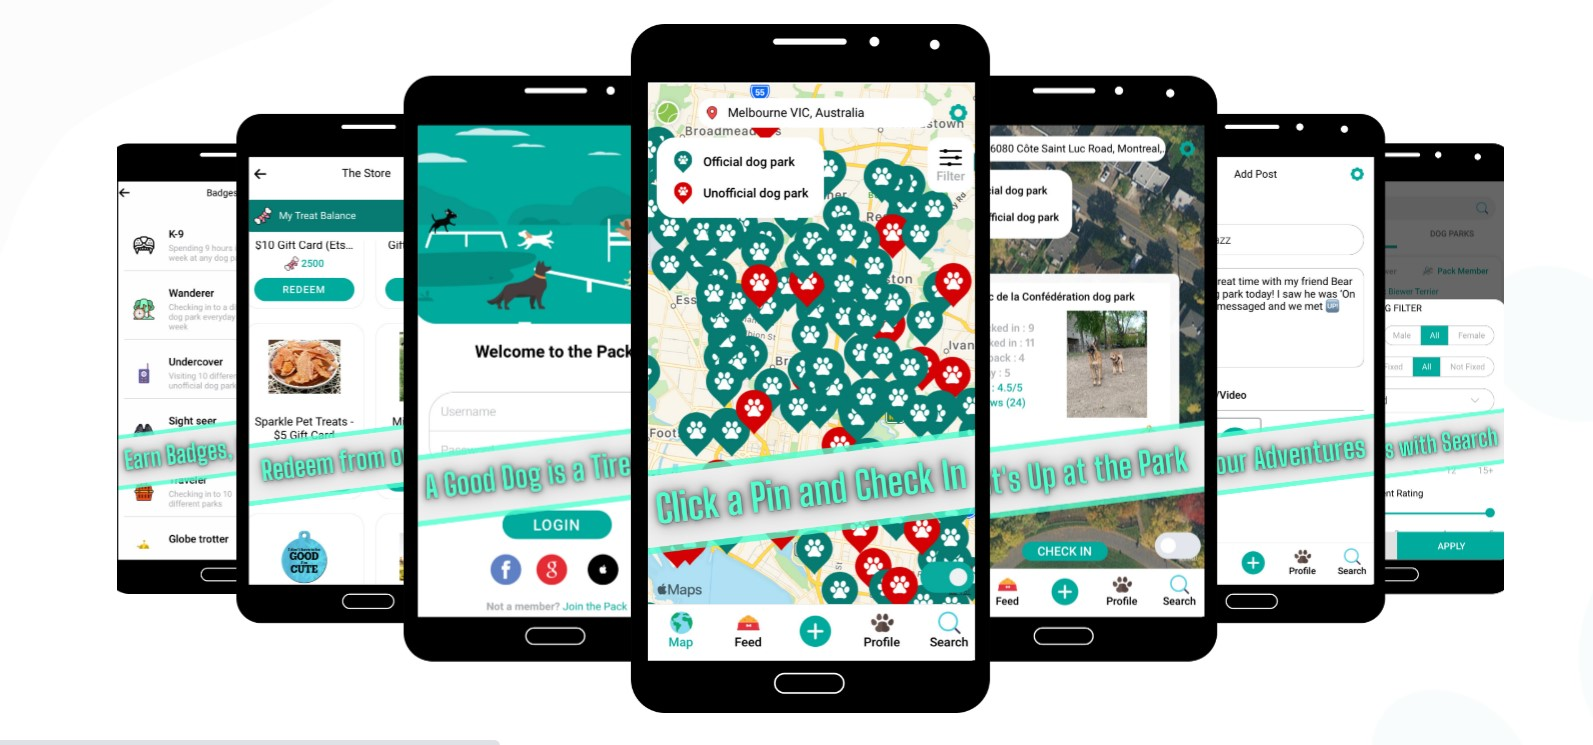
\includegraphics[width=\textwidth]{img/DogPack.jpg}
        \caption{Prikaz mogućnosti koje nudi aplikacija DogPack}
    \end{figure}
    
    
    \textbf{Dog Park Finder} \newline
    Aplikacija tvrtke Nylabone omogućuje korisnicima da unesu svoj poštanski broj i radius pretrage i aplikacija prikazuje na interaktivnoj karti lokacije svih parkova za pse u zadanom radiusu. Aplikacije je ograničena na korisnike iz SAD-a. 
    \begin{figure}[H]
        \centering
        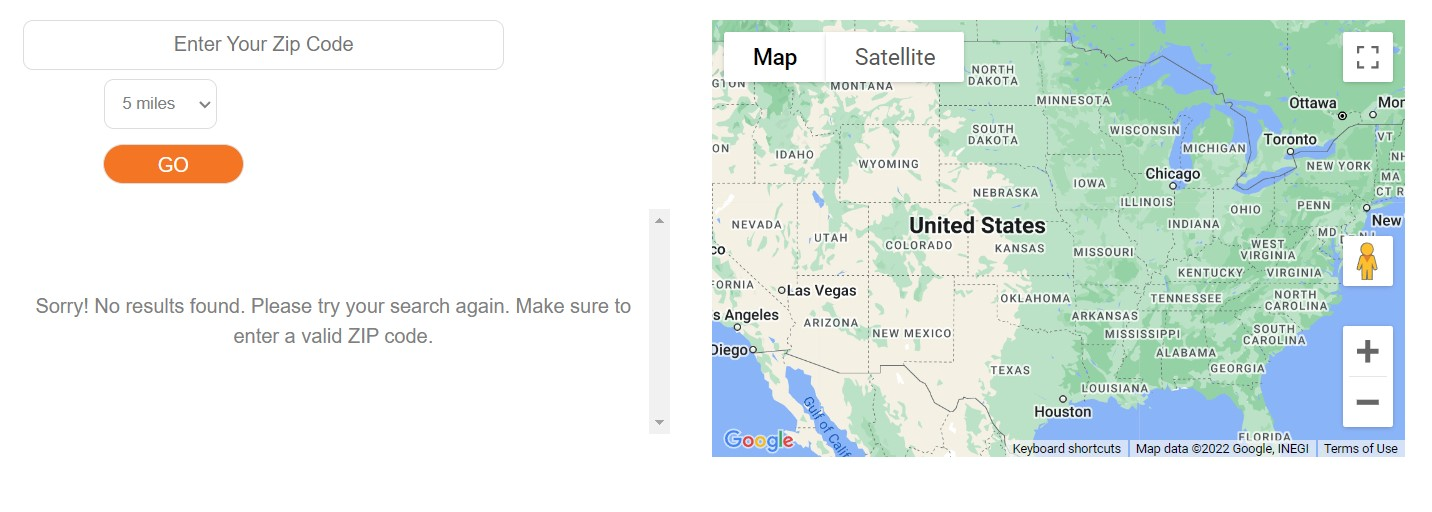
\includegraphics[width=\textwidth]{img/DogParkFinder.jpg}
        \caption{Prikaz karte}
    \end{figure}
    \textbf{Sniffspot} \newline
    Aplikacija omogućuje svojim korisnicima da unajme sigurne i privatne pseće parkove gdje možete sami sa svojim ljubimcem provoditi kvalitetno vrijeme. Aplikacija je ograničena na korisnike iz SAD-a.
    
	
		
		
		
		\chapter{Specifikacija programske potpore}

    \section{Funkcionalni zahtjevi}

    \noindent \textbf{Dionici:}
		\begin{packed_enum}
			\item Vlasnik obrta (naručitelj)
			\item Korisnici				
            \item Razvojni tim
		\end{packed_enum}
			
    \noindent \textbf{Aktori i njihovi funkcionalni zahtjevi:}
		\begin{packed_enum}
			\item  \underbar{Vlasnik obrta (inicijator) može:}
			\begin{packed_enum}
				\item dodati ili obrisati obrt
                \item dodati, izbrisati ili promijeniti
				\begin{packed_enum}
					\item  naziv i opis obrta
					\item  kategoriju lokacije 
				\end{packed_enum}
                \item  pregledavati i odgovarati na recenzije korisnika
                \item  pretplatom na aplikaciju osigurati neke dodatne pogodnosti poput reklame
			\end{packed_enum}
                
            \item  \underbar{Neregistrirani korisnik (inicijator) može:}
			\begin{packed_enum}
				\item pregledati na karti prikladno ili neprikladno označene lokacije za       pse, te plaćene lokacije koje su dodatno istaknute
                \item pretraživati specifičnu lokaciju ili odabrati kategoriju čiji se markeri onda prikazuju
                \item  odabirom markirane lokacije saznati više informacija o odabranom položaju (ime lokacije, ocjenu i  kategorija) ili u slučaju obrta (naziv obrta, ocjenu, tip obrta, opis obrta i kontakt)
                \item  se registrirati u sustav stvaranjem novog korisničkog računa
			\end{packed_enum}
            \eject

            \item  \underbar{Registrirani korisnik (inicijator) može:}
			\begin{packed_enum}
				\item označavati novu lokaciju što uključuje unos imena lokacije te odabir njene kategorije
                \item potvrditi ili negirati oznaku neke već postojeće lokacije
                \item pregledavati i mijenjati osobne podatke
                \item izbrisati svoj korisnički račun
                \item pisati recenziju i dati ocjenu  
			\end{packed_enum}
				
            \item  \underbar{Baza podataka (sudionik) može:}
			\begin{packed_enum}
				\item pohranjuje sve podatke o 
                \begin{packed_enum}
				    \item  korisnicima i njihovim ovlastima
				    \item  obrtima i njihovoj kategoriji
				\end{packed_enum}
			\end{packed_enum}
        \end{packed_enum}
	\eject 
    
    \subsection{Obrasci uporabe}
		\textbf{Opis obrazaca uporabe}
			
	    	\noindent\underbar{\textbf{UC1: Registracija korisnika}}
				\begin{itemize}
					\item \textbf{Glavni sudionik: } Korisnik 
					\item \textbf{Cilj: }Omogućiti korisniku prijavu u sustav, čime će korisnik ostvariti pravo na  korištenje više funkcijonalnosti aplikacije 
					\item \textbf{Sudionici: } Baza podataka 
					\item \textbf{Preduvjet: } - 
					\item \textbf{Opis osnovnog tijeka: }
					\begin{enumerate}
						\item Korisnik odabire opciju za registraciju
						\item Korisnik u registracijskom sučelju popunjava formu sa svojim podacima
						\item Korisnik dobiva e-mail na unesenu adresu u kojem potvrđuje svoju registraciju
					\end{enumerate}
					\item \textbf{Opis mogućih odstupanja:}
					\begin{itemize}
						\item Korisnik nije unio sve obavezne podatke
						\item Odabir već zauzetog korisničkog imena i/ili e-maila
						\item Unos podatka u nedozvoljenom formatu
					\end{itemize}
				\end{itemize}
					
			\noindent\underbar{\textbf{UC2: Prijava}}
				\begin{itemize}
					\item \textbf{Glavni sudionik: } Korisnik, vlasnik obrta 
					\item \textbf{Cilj: }Dobiti pristup korisničkom sučelju s dodatnim funkcionalnostima
					\item \textbf{Sudionici: } Baza podataka 
					\item \textbf{Preduvjet: } Uspješna registracija 
					\item \textbf{Opis osnovnog tijeka: }
					\begin{enumerate}
						\item Unos korisničkog imena i lozinke u formu za prijavu
						\item Potvrda o ispravnosti unešenih podataka
						\item Redirekcija na korisničko sučelje aplikacije
					\end{enumerate}
					\item \textbf{Opis mogućih odstupanja:}
					\begin{itemize}
						\item Pogrešno korisničko ime i/ili lozinka
					\end{itemize}
				\end{itemize}
					
			\noindent\underbar{\textbf{UC3: Pregled osobnih podataka}}
				\begin{itemize}
					\item \textbf{Glavni sudionik: } Korisnik, vlasnik obrta 
					\item \textbf{Cilj: }Omogućiti pregled osobnih podataka 
					\item \textbf{Sudionici: } Baza podataka 
					\item \textbf{Preduvjet: } Korisnik je prijavljen 
					\item \textbf{Opis osnovnog tijeka: }
					\begin{enumerate}
						\item Korisnik odabire opciju za prikaz osobnih podataka
						\item Prikaz osobnih podataka korisnika
					\end{enumerate}
				\end{itemize}
						
			\noindent\underbar{\textbf{UC4: Promjena osobnih podataka korisnika}}
				\begin{itemize}
					\item \textbf{Glavni sudionik: } Korisnik, vlasnik obrta 
					\item \textbf{Cilj: }Omogućiti promjenu korisničkog imena i/ili lozinke korisničkog računa 
					\item \textbf{Sudionici: } Baza podataka 
					\item \textbf{Preduvjet: } Korisnik je prijavljen 
					\item \textbf{Opis osnovnog tijeka: }
					\begin{enumerate}
						\item Korisnik odabire opciju za promjenom osobnih podataka
						\item Korisnik unosi nove osobne podatke i sprema promjene
						\item Promjene se spremaju u bazu podataka
					\end{enumerate}
					\item \textbf{Opis mogućih odstupanja:}
					\begin{itemize}
						\item Novo korisničko ime je zauzeto
					\end{itemize}
				\end{itemize}
					
			\noindent\underbar{\textbf{UC5: Brisanje korisničkog računa}}
				\begin{itemize}
					\item \textbf{Glavni sudionik: } Korisnik
					\item \textbf{Cilj: }Korisnik briše svoj korisnički račun
					\item \textbf{Sudionici: } Baza podataka 
					\item \textbf{Preduvjet: } Korisnik je prijavljen 
					\item \textbf{Opis osnovnog tijeka: }
					\begin{enumerate}
						\item Korisnik odabire opciju za brisanje svog korisničkog računa
						\item Odjava iz aplikacije
						\item Korisnički račun se briše iz baze podataka
						\item Redirekcija na naslovnu stranicu
					\end{enumerate}
				\end{itemize}
					
			\noindent\underbar{\textbf{UC6: Promjena podataka obrta}}
				\begin{itemize}
					\item \textbf{Glavni sudionik: } Vlasnik obrta 
					\item \textbf{Cilj: }Omogućiti vlasnicima obrta promjenu podataka o obrtima
					\item \textbf{Sudionici: } Baza podataka 
					\item \textbf{Preduvjet: } Vlasnik obrta je prijavljen
					\item \textbf{Opis osnovnog tijeka: }
					\begin{enumerate}
						\item Vlasnik obrta odabire opciju za promjenu podataka obrta
						\item Vlasnik mijenja ime, opis, kategoriju, OIB, kontakt broj i/ili neki drugi podatak
						\item Vlasnik sprema promjene
						\item Promjene se spremaju u bazu podataka
					\end{enumerate}
				\end{itemize}
					
			\noindent\underbar{\textbf{UC7: Brisanje računa vlasnika obrta}}
				\begin{itemize}
					\item \textbf{Glavni sudionik: } Vlasnik obrta 
					\item \textbf{Cilj: }Omogućiti vlasniku obrta brisanje računa
					\item \textbf{Sudionici: } Baza podataka 
					\item \textbf{Preduvjet: } Vlasnik obrta je prijavljen
					\item \textbf{Opis osnovnog tijeka: }
					\begin{enumerate}
						\item Vlasnik obrta odabire opciju za brisanje računa
						\item Odjava iz aplikacije
						\item Račun vlasnika obrta se briše iz baze podataka
                        \item Redirekcija na naslovnu stranicu
					\end{enumerate}
				\end{itemize}
					
			\noindent\underbar{\textbf{UC8: Pregled podataka lokacije}}
				\begin{itemize}
					\item \textbf{Glavni sudionik: } Korisnik, vlasnik obrta 
					\item \textbf{Cilj: }Pregled podataka bilo koje unesene lokacije
					\item \textbf{Sudionici: } Baza podataka 
					\item \textbf{Preduvjet: } -
					\item \textbf{Opis osnovnog tijeka: }
					\begin{enumerate}
						\item Učitava se karta sa unesenim lokacijama
						\item Klikom na pojedinu lokaciju prikazuju se njeni podaci
					\end{enumerate}
				\end{itemize}
					
			\noindent\underbar{\textbf{UC9: Potvrđivanje ili negiranje oznake postojeće lokacije}}
				\begin{itemize}
					\item \textbf{Glavni sudionik: } Korisnik, vlasnik obrta 
					\item \textbf{Cilj: }Omogućiti prijavljenim korisnicima da potvrde ili negiraju oznaku postojeće lokacije
					\item \textbf{Sudionici: } Baza podataka 
					\item \textbf{Preduvjet: } Korisnik ili vlasnik obrta su prijavljeni
					\item \textbf{Opis osnovnog tijeka: }
					\begin{enumerate}
						\item Kod prikaza informacija pojedine lokacije, korisnik odabire opciju potvrđivanja ili negiranja lokacije
						\item Informacija se sprema u bazu podataka
					\end{enumerate}
				\end{itemize}
					
			\noindent\underbar{\textbf{UC10: Označavanje novih lokacija}}
				\begin{itemize}
					\item \textbf{Glavni sudionik: } Korisnik, vlasnik obrta 
					\item \textbf{Cilj: }Omogućiti unos neke lokacije koja je (ne)prikladna za pse
					\item \textbf{Sudionici: } Baza podataka 
					\item \textbf{Preduvjet: } Korisnik ili vlasnik obrta su prijavljeni
					\item \textbf{Opis osnovnog tijeka: }
					\begin{enumerate}
						\item Korisnik odabire opciju za označavanjem nove lokacije
						\item Korisnik unosi ime i kategoriju lokacije te je li ona prikladna za pse
						\item Podaci se spremaju u bazu podataka
					\end{enumerate}
				\end{itemize}
					
			\noindent\underbar{\textbf{UC11: Prikaz lokacija po odabranoj kategoriji}}
				\begin{itemize}
					\item \textbf{Glavni sudionik: } Korisnik, vlasnik obrta 
					\item \textbf{Cilj: }Omogućiti prikaz lokacija na karti po odabranoj kategoriji
					\item \textbf{Sudionici: } Baza podataka 
					\item \textbf{Preduvjet: } -
					\item \textbf{Opis osnovnog tijeka: }
					\begin{enumerate}
						\item Korisnik na karti odabire kategoriju po kojoj želi filtrirati lokacije
						\item Na karti se prikazuju samo lokacije sa odabranom kategorijom
					\end{enumerate}
				\end{itemize}		
				
			\noindent\underbar{\textbf{UC12: Registracija vlasnika obrta}}
				\begin{itemize}
					\item \textbf{Glavni sudionik: } Vlasnik obrta 
					\item \textbf{Cilj: }Omogućiti vlasniku obrta prijavu u sustav, čime će vlasnik obrta ostvariti pravo na korištenje više funkcijonalnosti aplikacije
					\item \textbf{Sudionici: } Baza podataka 
					\item \textbf{Preduvjet: } -
					\item \textbf{Opis osnovnog tijeka: }
					\begin{enumerate}
			    		\item Vlasnik obrta odabire opciju za registraciju
						\item Vlasnik obrta u registracijskom sučelju popunjava formu sa svojim podacima i podacima obrta
                        \item Vlasnik obrta na unesenu e-mail adresu dobiva potvrdu o uspješnoj registraciji i uspješnom plaćanju
					\end{enumerate}
                    \item \textbf{Opis mogućih odstupanja:}
					\begin{itemize}
						\item Vlasnik obrta nije unio sve obavezne podatke
						\item Odabir već zauzetog korisničkog imena i/ili e-maila
						\item Unos podatka u nedozvoljenom formatu
					\end{itemize}
				\end{itemize}

            \noindent\underbar{\textbf{UC13: Pisanje recenzija i davanje ocjena lokacijama i obrtima}}
				\begin{itemize}
					\item \textbf{Glavni sudionik: } Korisnik
					\item \textbf{Cilj: }Napisati recenziju i ocijeniti lokaciju ili obrt
					\item \textbf{Sudionici: } Baza podataka 
					\item \textbf{Preduvjet: } Korisnik je prijavljen
					\item \textbf{Opis osnovnog tijeka: }
					\begin{enumerate}
						\item Korisnik napiše recenziju i ocijeni lokaciju ili obrt
						\item Ocjena i recenzija se pohranjuju u bazu podataka i ažurira se prosječna ocjena lokacije ili obrta 
					\end{enumerate}
                    \item \textbf{Opis mogućih odstupanja:}
					\begin{itemize}
						\item Korisnik ne želi napisati osvrt
					\end{itemize}
				\end{itemize} 

            \noindent\underbar{\textbf{UC14: Pregled recenzija korisnika}}
			    \begin{itemize}
					\item \textbf{Glavni sudionik: } Vlasnik obrta
					\item \textbf{Cilj: }Pregledati recenzije korisnika za vlasnikov obrt 
					\item \textbf{Sudionici: } Baza podataka 
					\item \textbf{Preduvjet: } Vlasnik obrta je prijavljen
					\item \textbf{Opis osnovnog tijeka: }
					\begin{enumerate}
						\item Vlasnik odabire opciju “Pregledaj recenzije“
						\item Prikažu se sve dotadašnje recenzije i ocjene vlasnikovog obrta
					\end{enumerate}
				\end{itemize} 	
			
	\pagebreak
	\subsection*{Dijagrami obrazaca uporabe}
    	\begin{figure}[H]
            \centering                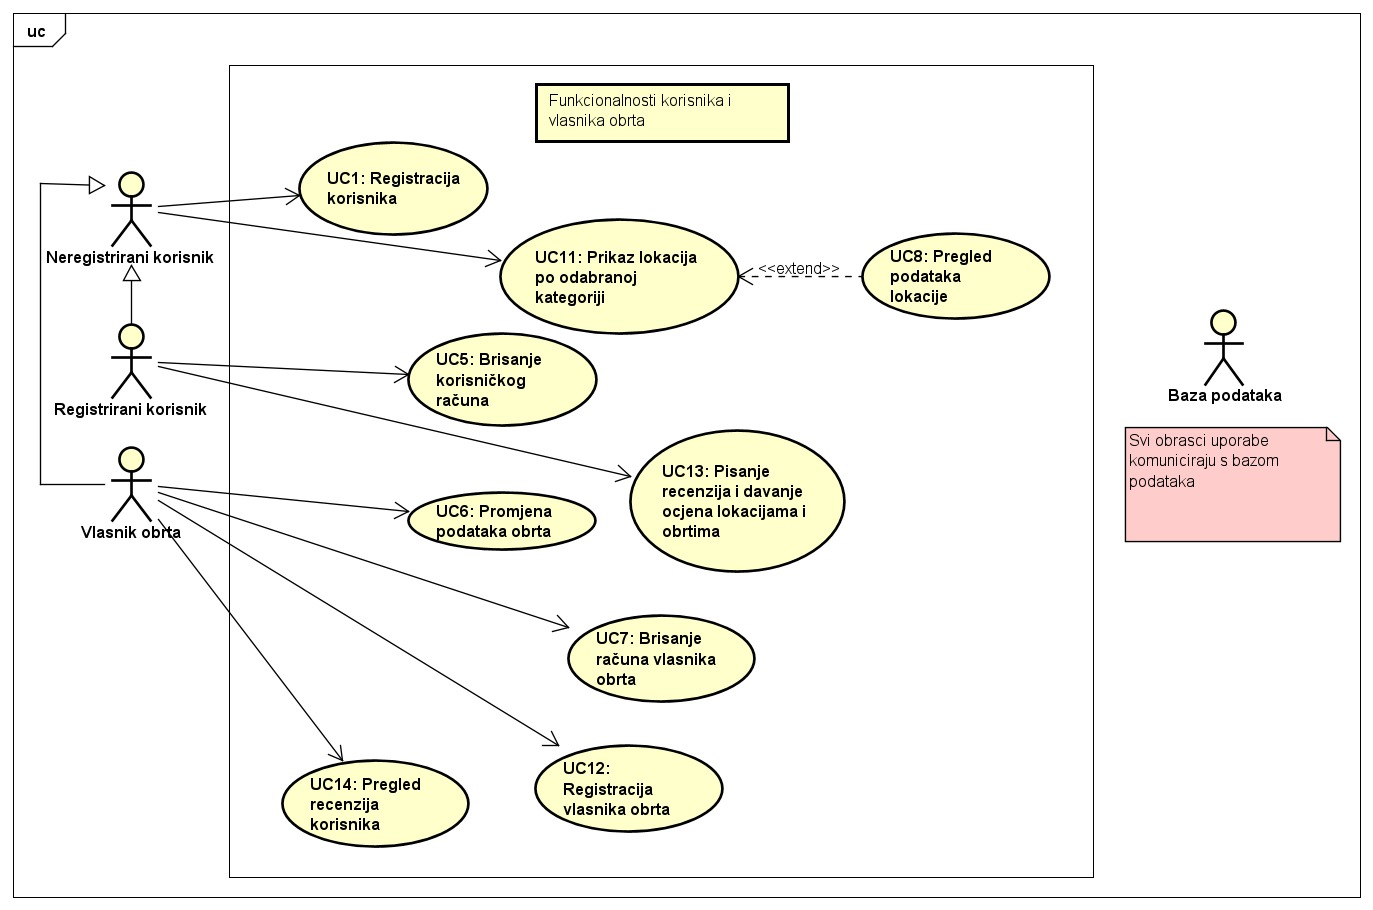
\includegraphics[width=\textwidth]{img/UseCaseDiagram1.png}
            \caption{Funkcionalnost korisnika i vlasnika obrta}
        \end{figure}
		\begin{figure}[H]
			\centering
			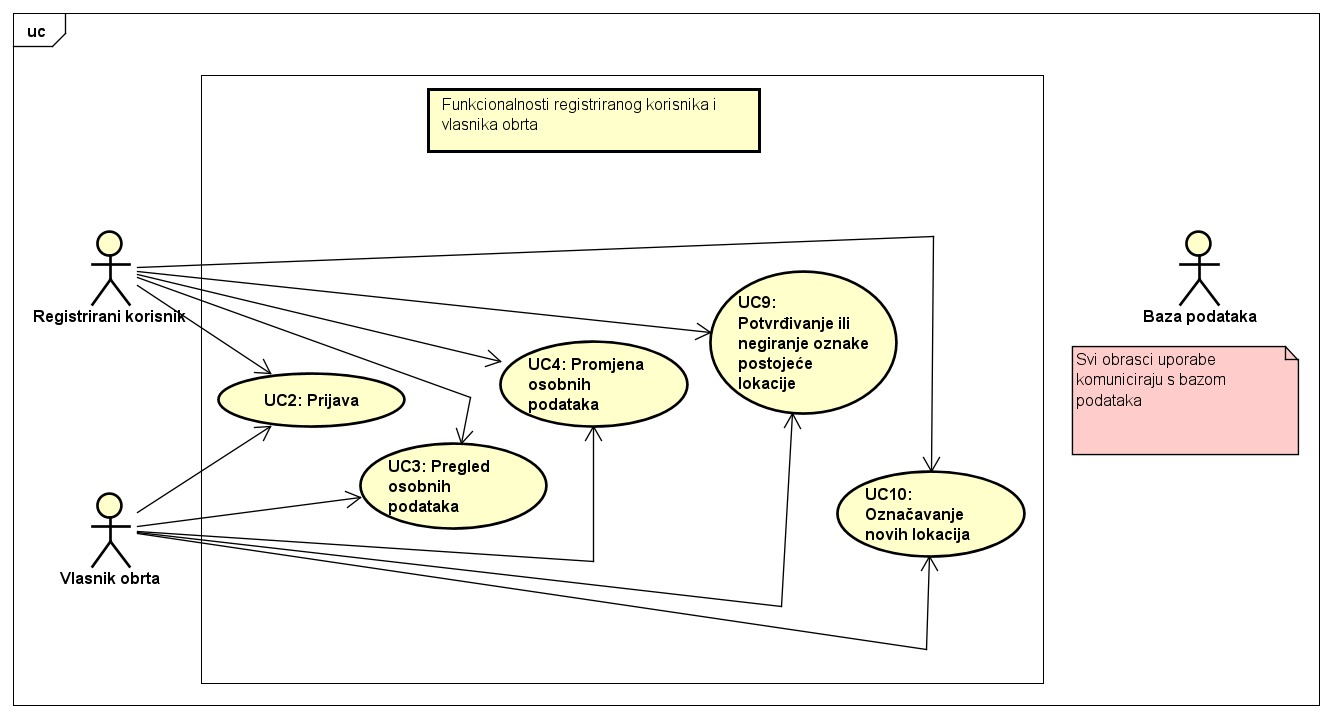
\includegraphics[width=\textwidth]{img/UseCaseDiagram2.png}
			\caption{Funkcionalnost registriranog korisnika i vlasnika obrta}
			    \end{figure}

    \subsection{Sekvencijski dijagrami}
		\textbf{Obrasci uporabe UC1 i UC12 - Registracija}
				
		Korisnik ili vlasnik obrta šalje zahtjev za registracijom koji za osnovne korisnike sadrži e-mail adresu, korisničko ime, lozinku, ime, prezime i opis. Zahtjev za registraciju vlasnika obrta sadrži e-mail adresu, lozinku te naziv, adresu, OIB, kontakt broj, djelatnost i kratki opis obrta. Web aplikacija validira ulazne podatke te se podaci spremaju u bazu podataka. Korisniku se nakon toga na navedenu e-mail adresu šalje link za verifikaciju računa.
			\begin{figure}[H]
				\centering
				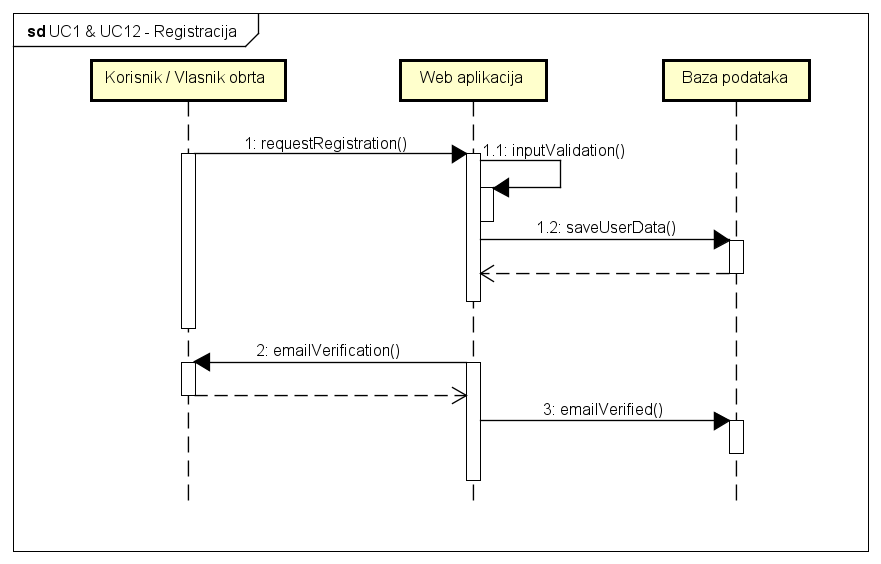
\includegraphics[width=\textwidth]{img/UC1&UC12-Registracija.png}
				\caption{Sekvencijski dijagram registracije korisnika ili vlasnika obrta}
			\end{figure}
			
			\pagebreak \noindent \textbf{Obrazac uporabe UC9 - Potvrđivanje ili negiranje oznake postojeće lokacije}
			
			Korisnik ili vlasnik obrta šalje zahtjev za učitavanjem karte na naslovnoj stranici, podaci se povlače iz baze podataka te se lokacije iscrtavaju na karti. Klikom na neku od lokacija korisniku se prikazuju osnovni podaci odabrane lokacije ili obrta. Ukoliko je korisnik(ili vlasnik obrta) prijavljen, on može potvrditi ili negirati postojanje označene lokacije, što će se zatim spremiti u bazu podataka.
			\begin{figure}[H]
				\centering
				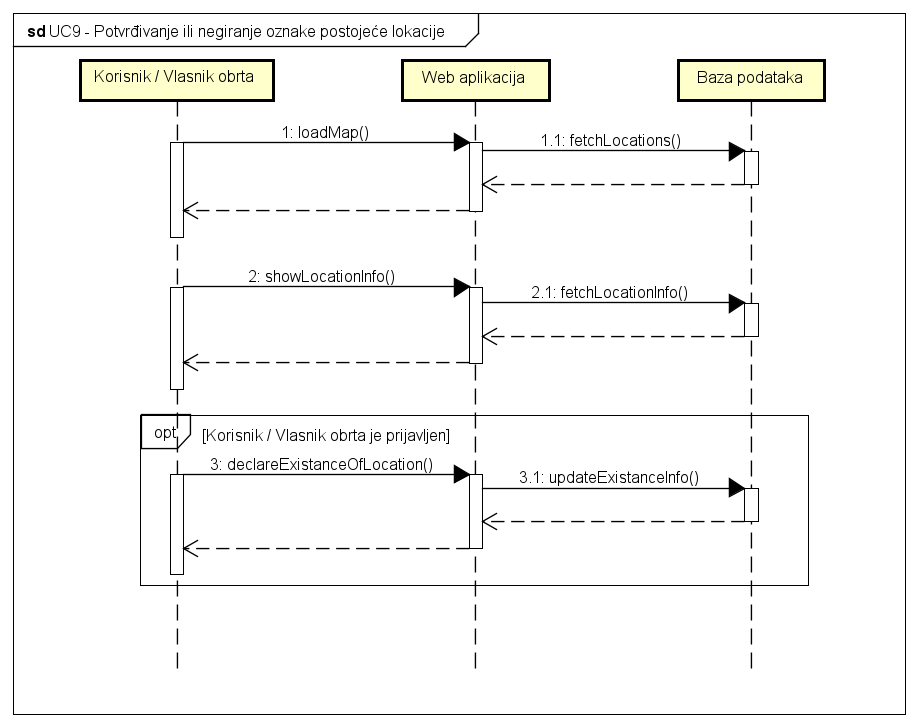
\includegraphics[width=\textwidth]{img/UC9-Potvrdivanje_ili_negiranje_oznake_postojece_lokacije.png}
				\caption{Sekvencijski dijagram potvrđivanja ili negiranja postojećih lokacija}
			\end{figure}
			
			\pagebreak \noindent \textbf{Obrazac uporabe UC10 - Označavanje novih lokacija}
			
			Korisnik prilikom učitavanja naslovne stranice šalje zahtjev za učitavanjem karte s lokacijama, uslijed čega web aplikacija povlači iz baze podataka potrebne podatke o lokacijama te ih iscrtava na karti. Registrirani i prijavljeni korisnik može označiti novu lokaciju na karti te za nju navesti ime lokacije, kategoriju te je li prikladna za pse. Uneseni podaci se spremaju u bazu podataka.
			\begin{figure}[H]
				\centering
				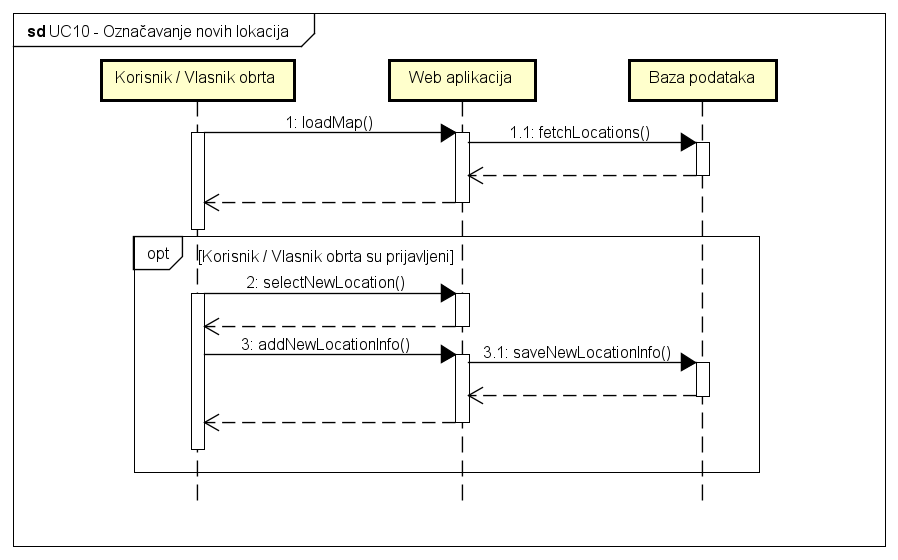
\includegraphics[width=\textwidth]{img/UC10-Oznacavanje_novih_lokacija.png}
				\caption{Sekvencijski dijagram označavanja novih lokacija}
			\end{figure}
			
			\pagebreak \noindent \textbf{Obrazac uporabe UC13 - Pisanje recenzija i ocjenjivanje lokacija}
			
			Korisniku se klikom na marker lokacije prikazuju osnovni podaci unesene lokacije ili obrta. Nadalje, korisnik može poslati zahtjev za recenzijama odabrane lokacije koje se zatim povlače iz baze podataka. Ukoliko je korisnik prijavljen, on može napisati vlastitu recenziju i/ili ocijeniti lokaciju s jednom do pet zvjezdica. Napisana recenzija i/ili odabrana ocjena se zatim spremaju u bazu podataka.
			
			\begin{figure}[H]
				\centering
				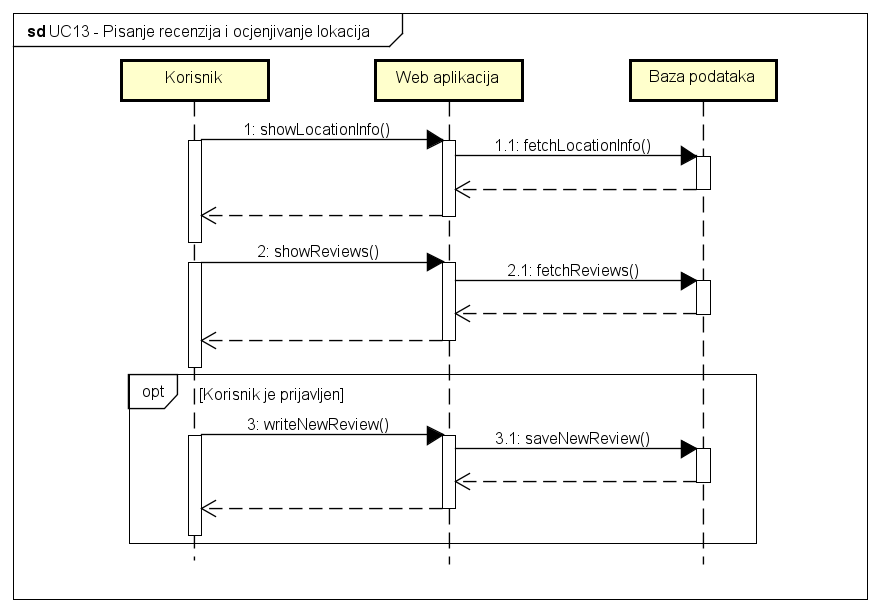
\includegraphics[width=\textwidth]{img/UC13-Pisanje_recenzija_i_ocjenjivanje_lokacija.png}
				\caption{Sekvencijski dijagram pisanja recenzija i ocjenjivanja lokacija}
			\end{figure}
    
    \pagebreak \section{Ostali zahtjevi}
	\begin{itemize}
		\item Dohvaćanje podataka iz baze podataka ne smije trajati dulje od nekoliko sekundi
		\item Lozinke i ostali povjerljivi podaci u bazi podataka moraju biti kriptirani
		\item Neispravno korištenje korisničkog sučelja i neispravan unos podataka ne smiju narušiti funkcionalnost aplikacije i integritet baze podataka
		\item Sustav treba biti implementiran kao web aplikacija koristeći objektno-orijentirane jezike
		\item Sustav treba funkcionirati pri istovremenom korištenju više korisnika
		\item Korisničko sučelje treba biti jednostavno i intuitivno za korištenje
		\item Nadogradnje sustava ne smiju narušavati postojeće funkcionalnosti sustava
		\item Veza s bazom podataka mora biti kvalitetno zaštićena, brza i otporna na vanjske greške
		\item Pristup sustavu mora biti omogućen iz javne mreže pomoću HTTPS
	\end{itemize}
		\chapter{Arhitektura i dizajn sustava}

    \hfill\break
    Arhitektura se može podijeliti na tri podsustava: 
    \begin{itemize}
		\item \textbf{Web poslužitelj} 
		\item \textbf{Web aplikacija } 
		\item \textbf{Baza podataka } 
	\end{itemize}
	\hfill\break	
	
	\textbf{Web preglednik} je aplikacija za pristup World Wide Web-u. Kada korisnik želi otvoriti web stranicu, web preglednik šalje HTTP protokol preko kojega zahtjeva sadržaj stranice. Nakon što dobije sadržaj stranice web preglednik ga prevodi i prikazuje korisniku kao jasno i razumljivo grafičko sučelje. 
	\newline \newline
	
	\textbf{Web poslužitelj} je računalo na kojem se izvodi aplikacija.Njegova glavna zadaća je prihvaćanje zahtjeva putem HTTP protokola. Poslužitelj šalje zahtjeve web aplikaciji na obradu i korisniku vraća odgovor.
	\newline \newline
	
	\textbf{Web aplikacija} je zaslužna za obradu korisničkih zahtjeva. Ima pristup bazi podataka. Odgovore šalje u obliku HTML dokumenta web poslužitelju koji ih prosljeđuje korisniku. Arhitektura aplikacije se može podijeliti na front-end i back-end. Cijeli sustav se poslužuje pomoću \textbf{digitalOcean-a}
	\newline\newline
	
	Za izradu backend dijela naše aplikacije odabrali smo radni okvir Spring Boot. Programski jezik koji koristimo je Java.\newline Struktura toga dijela aplikacije biti će troslojna:
	\begin{itemize}
		\item \textbf{Controller} je sloj na kojem se nalazi naš REST API
		\item \textbf{Service} sloj upravlja poslovnom logikom naše aplikacije
		\item \textbf{Repository} sloj služi za pristup podatcima u bazi podataka
	\end{itemize}
					    
	\begin{figure}[H]
        \centering
        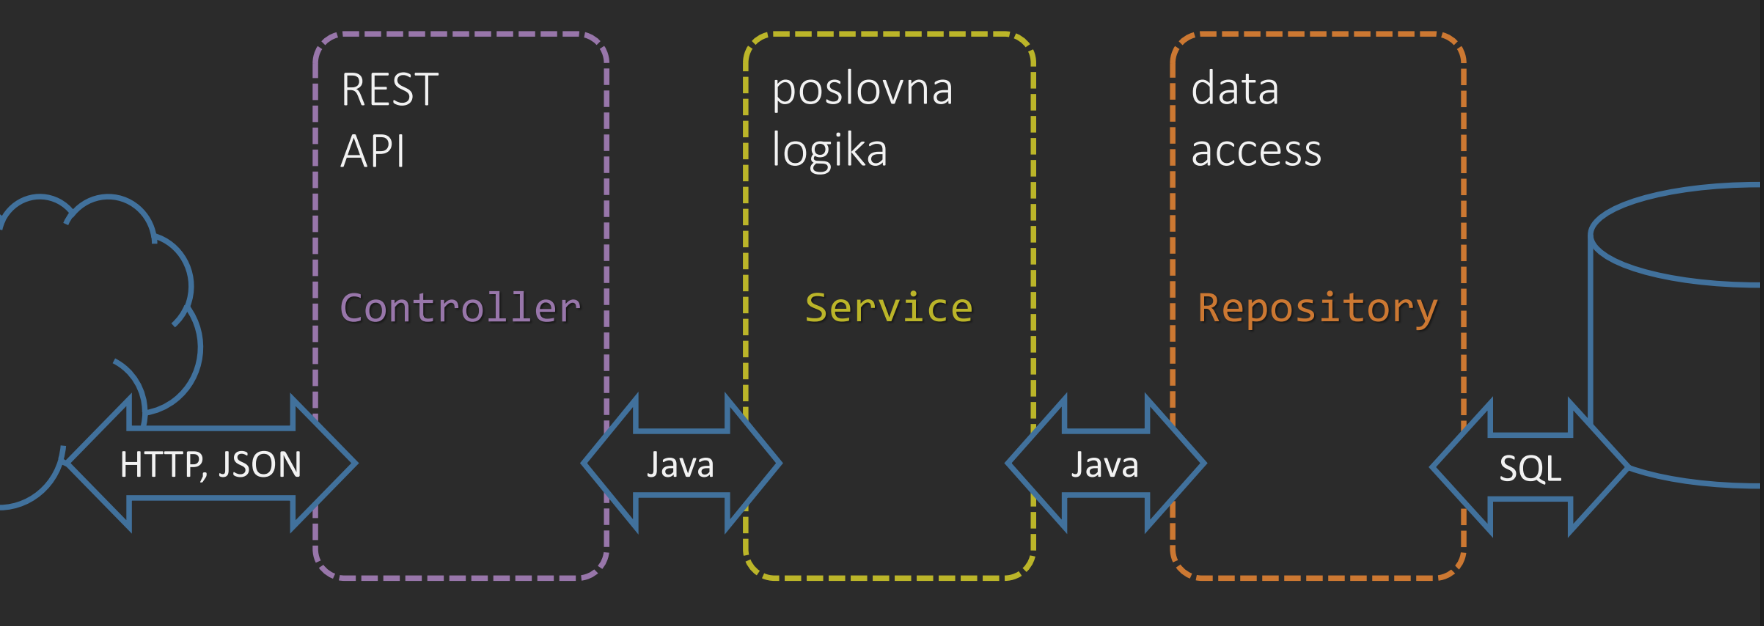
\includegraphics[width=\textwidth]{img/SpringBootflowArchitecture.png}
        \caption{Prikaz troslojne strukture Spring Boot radnog okvira}
    \end{figure}
	\hfill\break
	Za izradu frontend dijela naše aplikacije odabrali smo Javascript library React. Uz React su nam potrebni i alat node.js te upravitelj paketa npm.  

    \section{Baza podataka}
    Analizom zahtjeva utvrđeno je da aplikacija treba podržavati više korisnika koji istodobno mogu pregledavati, uređivati, stvarati i/ili brisati podatke bez da se pojave nekonzistentnosti. Podatci koje je potrbeno spremati, unaprijed su poznati i dobro definirani, a nisu prirodno strukturirani kao graf pa je relacijska baza podataka izabrana kao najbolje rješenje za pohranu podataka.Za bazu podataka smo koristili Postgresql.
    \eject
    
    \subsection{Opis tablica}
        \hfill\break
        Entitet Račun sadrži informacije koje su iste za svakog korisnika i koje korisnik unosi prilikom registracije. Atributi računa su: ID računa koji se dodijeljuje automatski, email, lozinku, opis, vrsta korisnika (osnovni ili vlasnik obrta). Atribut zaključano je postavljen na false, a mijenja se na true ako korisnik više puta pogriješi lozinku. Omogućeno se postavlja na true ako je račun aktivan.
        \hfill\break
	    \begin{tblr}{
                hlines = {},
                colspec={|X[9,l]|X[7, l]|X[15, l]|}, 
                cell{1}{1} = {c = 3}{halign = c}
            }
            {\bf account} (Račun) &    &    \\
            \SetRow{LightGreen} account\textunderscore id & INT & identifikator  \\
            email & VARCHAR(50) & adresa e-pošte \\
            password & VARCHAR(60) & enkriptirana lozinka \\
            bio & VARCHAR(200) & biografija \\
            user\textunderscore role & VARCHAR(10) & razina autorizacije korisnika \\
            locked & BOOLEAN & istina ako korisnik više puta unese pogršnu lozinku \\
            enabled & BOOLEAN & istina ako je račun aktivan 
        \end{tblr}
        \hfill\break
        
        Nakon ispunjavanja registracijske forme korisnik na mail dobiva link kojim potvrđuje račun. Ta potvrda se sprema u tablicu Token za potvrdu računa. Tablica sadrži atribute ID tokena za potvrdu, token za potvrdu, datum kreiranja u kojima se bilježe podatci o tokenu te ID računa potreban da se poveže s računom koji se aktivira.
        \hfill\break
        \begin{tblr}{
                hlines = {},
                colspec={|X[9,l]|X[7, l]|X[15, l]|}, 
                cell{1}{1} = {c = 3}{halign = c}
            }
            {\bf confirmation\textunderscore token } (Token za potvrdu računa) &    &    \\
            \SetRow{LightGreen} confirmation\textunderscore token\textunderscore id & INT & identifikator  \\
            confirmation\textunderscore token & VARCHAR(36) & token za potvrdu računa\\
            created\textunderscore date & DATE & datum kreiranja tokena \\
            \SetRow{LightBlue} account\textunderscore id & INT & iden. računa za koji je vezan token \\
        \end{tblr}
        \hfill\break
        
        Tablica Korisnički račun sadrži atribute vezane uz osnovnog korisnika. Atribut ID računa posuđen je iz tablice račun uz koji se veže. Dodatni atributi su još korisničko ime, ime i prezime.
        \hfill\break
        \begin{tblr}{
                hlines = {},
                colspec={|X[9,l]|X[7, l]|X[15, l]|}, 
                cell{1}{1} = {c = 3}{halign = c}
            }
            {\bf user\textunderscore account} (Korisnički račun) &    &    \\
            \SetRow{LightGreen} account\textunderscore id & INT & posuđeni ključ  \\
            username & VARCHAR(30) & korisiničko ime \\
            first\textunderscore name & VARCHAR(30) & ime \\
            last\textunderscore name & VARCHAR(30) & prezime 
        \end{tblr}
        \hfill\break
        
        Poslovni račun je tablica za drugi tip korisnika. Također od entiteta račun posuđuje atribut ID računa, a uz njega još sadrži ime obrta, OIB, kontakt broj i ID tipa obrta.
        \hfill\break
        \begin{tblr}{
                hlines = {},
                colspec={|X[9,l]|X[7, l]|X[15, l]|}, 
                cell{1}{1} = {c = 3}{halign = c}
            }
            {\bf business\textunderscore account} (Poslovni račun) &    &    \\
            \SetRow{LightGreen} account\textunderscore id & INT & posuđeni ključ  \\
            business\textunderscore name & VARCHAR(30) & ime obrta \\
            oib & CHAR(11) & oib \\
            phone\textunderscore number & VARCHAR(15) & broj telefona \\
            \SetRow{LightBlue} business\textunderscore type\textunderscore id & INT & ključ relacije bussinesType \\
        \end{tblr}
        \hfill\break

        Tablica lista obrta povezana je preko atributa ID tipa obrta s poslovnim računom i u nju se sprema tip obrta.
        \hfill\break
        \begin{tblr}{
                hlines = {},
                colspec={|X[9,l]|X[7, l]|X[15, l]|}, 
                cell{1}{1} = {c = 3}{halign = c}
            }
            {\bf business\textunderscore type} (Vrsta obrta) &    &    \\
            \SetRow{LightGreen} business\textunderscore type\textunderscore id & INT & identifikator  \\
            business\textunderscore type & VARCHAR(30) & vrsta obrta
        \end{tblr}
        \hfill\break

        Tablica Lokacija sadrži atribut ID lokacije koji nam je potreban za povezivanje ostalih entiteta vezanih uz lokaciju. Osim toga sadrđi još atribute za geografsku dužinu i širinu, adresu, ime lokacije i njezin opis, datum i vrijeme kreiranja. Atribut promovirana je postavljen na nulu osim ako se radi o promoviranoj lokaciji (obrt). Atribut "dog friendly" je boolean koji je true ako je lokacija prikladna za pse. U tablici se također sprema i ID računa korisnika koji ju je kreirao te se još postavlja ID tipa lokacije.
        \hfill\break
        \begin{tblr}{
                hlines = {},
                colspec={|X[9,l]|X[7, l]|X[15, l]|}, 
                cell{1}{1} = {c = 3}{halign = c}
            }
            {\bf location} (Lokacija) &    &    \\
            \SetRow{LightGreen} location\textunderscore id & INT & identifikator  \\
            longitude & NUMERIC(8,5) & longituda \\
            latitude & NUMERIC(8,5) & latituda \\
            address & VARCHAR(50) & adresa \\
            location\textunderscore name & VARCHAR(30) & ime lokacije \\
            location\textunderscore description & VARCHAR(200) & opis lokacije \\
            date\textunderscore time\textunderscore created & TIMESTAMP & vrijeme i datum objave lokacije \\
            promoted & INT & nije nula ako je lokacija promovirana\\
            dog\textunderscore friendly & BOOLEAN & je li lokacija prikladna za pse \\
            account\textunderscore id & INT & identifikator korisnika koji je stvorio lokaciju \\
            \SetRow{LightBlue} location\textunderscore type\textunderscore id & INT & identifikator vrste lokacije
        \end{tblr}
        \hfill\break

        Tip lokacije je tablica koja se preko atributa ID tipa lokacije povezuje se prethodnom tablicom, a dodatno još ima atribut tip lokacije u koji se on upisuje.
        \hfill\break
        \begin{tblr}{
                hlines = {},
                colspec={|X[9,l]|X[7, l]|X[15, l]|}, 
                cell{1}{1} = {c = 3}{halign = c}
            }
            {\bf location\textunderscore type} (Tip lokacije) &    &    \\
            \SetRow{LightGreen} location\textunderscore type\textunderscore id & INT & identifikator  \\
            location\textunderscore type & VARCHAR(30) & vrsta lokacije
        \end{tblr}
        \hfill\break

        Posljednja tablica je Ocjena. U nju se spremaju atributi potrebi za prikaz ocjene određene lokacije. Preko atributa ID lokacije se povezuje s lokacijom na koju se odnosi, a ID računa zapisuje tko je postavio tu ocjenu. Ostali atributi su vrijeme i datum kreiranja, broj zvijezdica i poruka uz ocjenu.
        \hfill\break
        \begin{tblr}{
                hlines = {},
                colspec={|X[9,l]|X[7, l]|X[15, l]|}, 
                cell{1}{1} = {c = 3}{halign = c}
            }
            {\bf review} (Ocjena) &    &    \\
            \SetRow{LightGreen} location\textunderscore id & INT & idn. lokacije za koju je napisana ocjena  \\
            \SetRow{LightGreen} account\textunderscore id & VARCHAR(30) & idn. korinika koji je napisao ocjenu \\
            date\textunderscore time\textunderscore created & TIMESTAMP & vrijeme i datum objave ocjene \\
            stars & FLOAT & ocjena lokacije između 1 i 5 \\
            message & VARCHAR(200) & tekst ocjene
        \end{tblr}
				
			
	\subsection{Dijagram baze podataka}
		\begin{figure}[H]
    		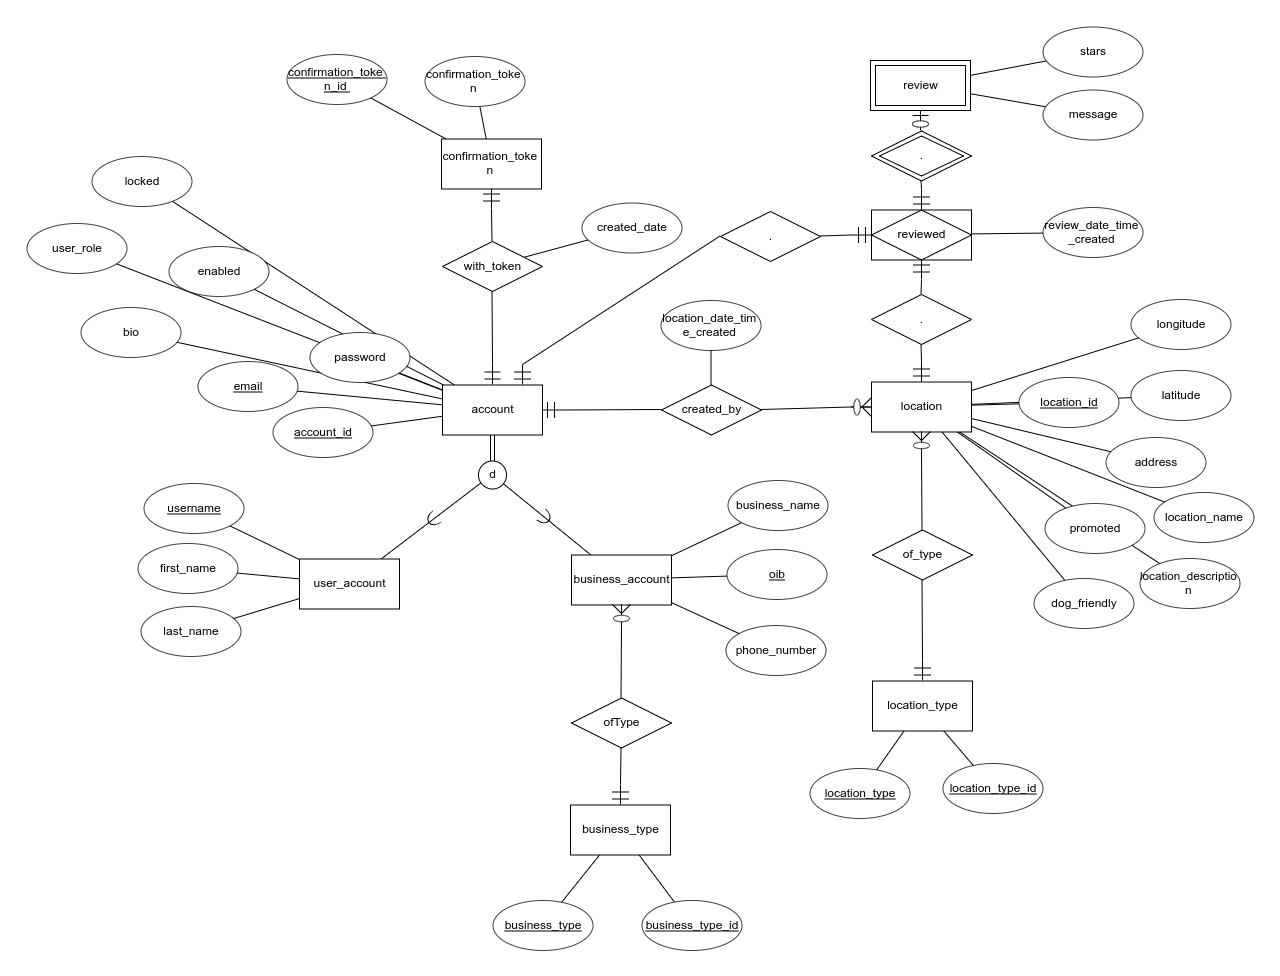
\includegraphics[width=\textwidth]{img/er_dijagram.png}
    		\centering
    		\caption{ER dijagram baze podataka}
    		\label{fig:promjene}
    	\end{figure}

        \begin{figure}[H]
    		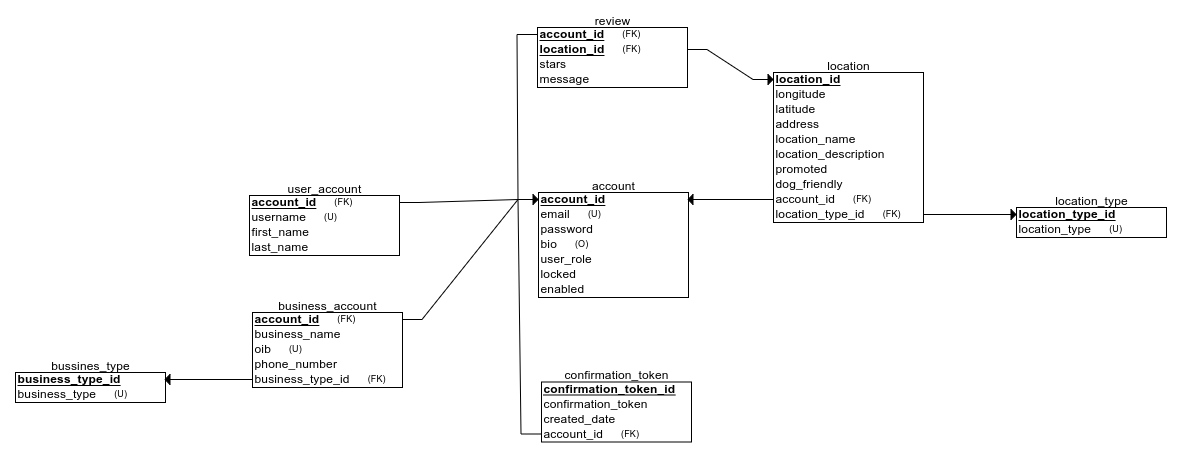
\includegraphics[width=\textwidth]{img/rel_dijagram.png}
    		\centering
    		\caption{Relacijski dijagram baze podataka}
    		\label{fig:promjene}
    	\end{figure}
			
	\eject
        
    
    \section{Dijagram razreda}
        \begin{figure}[H]
        	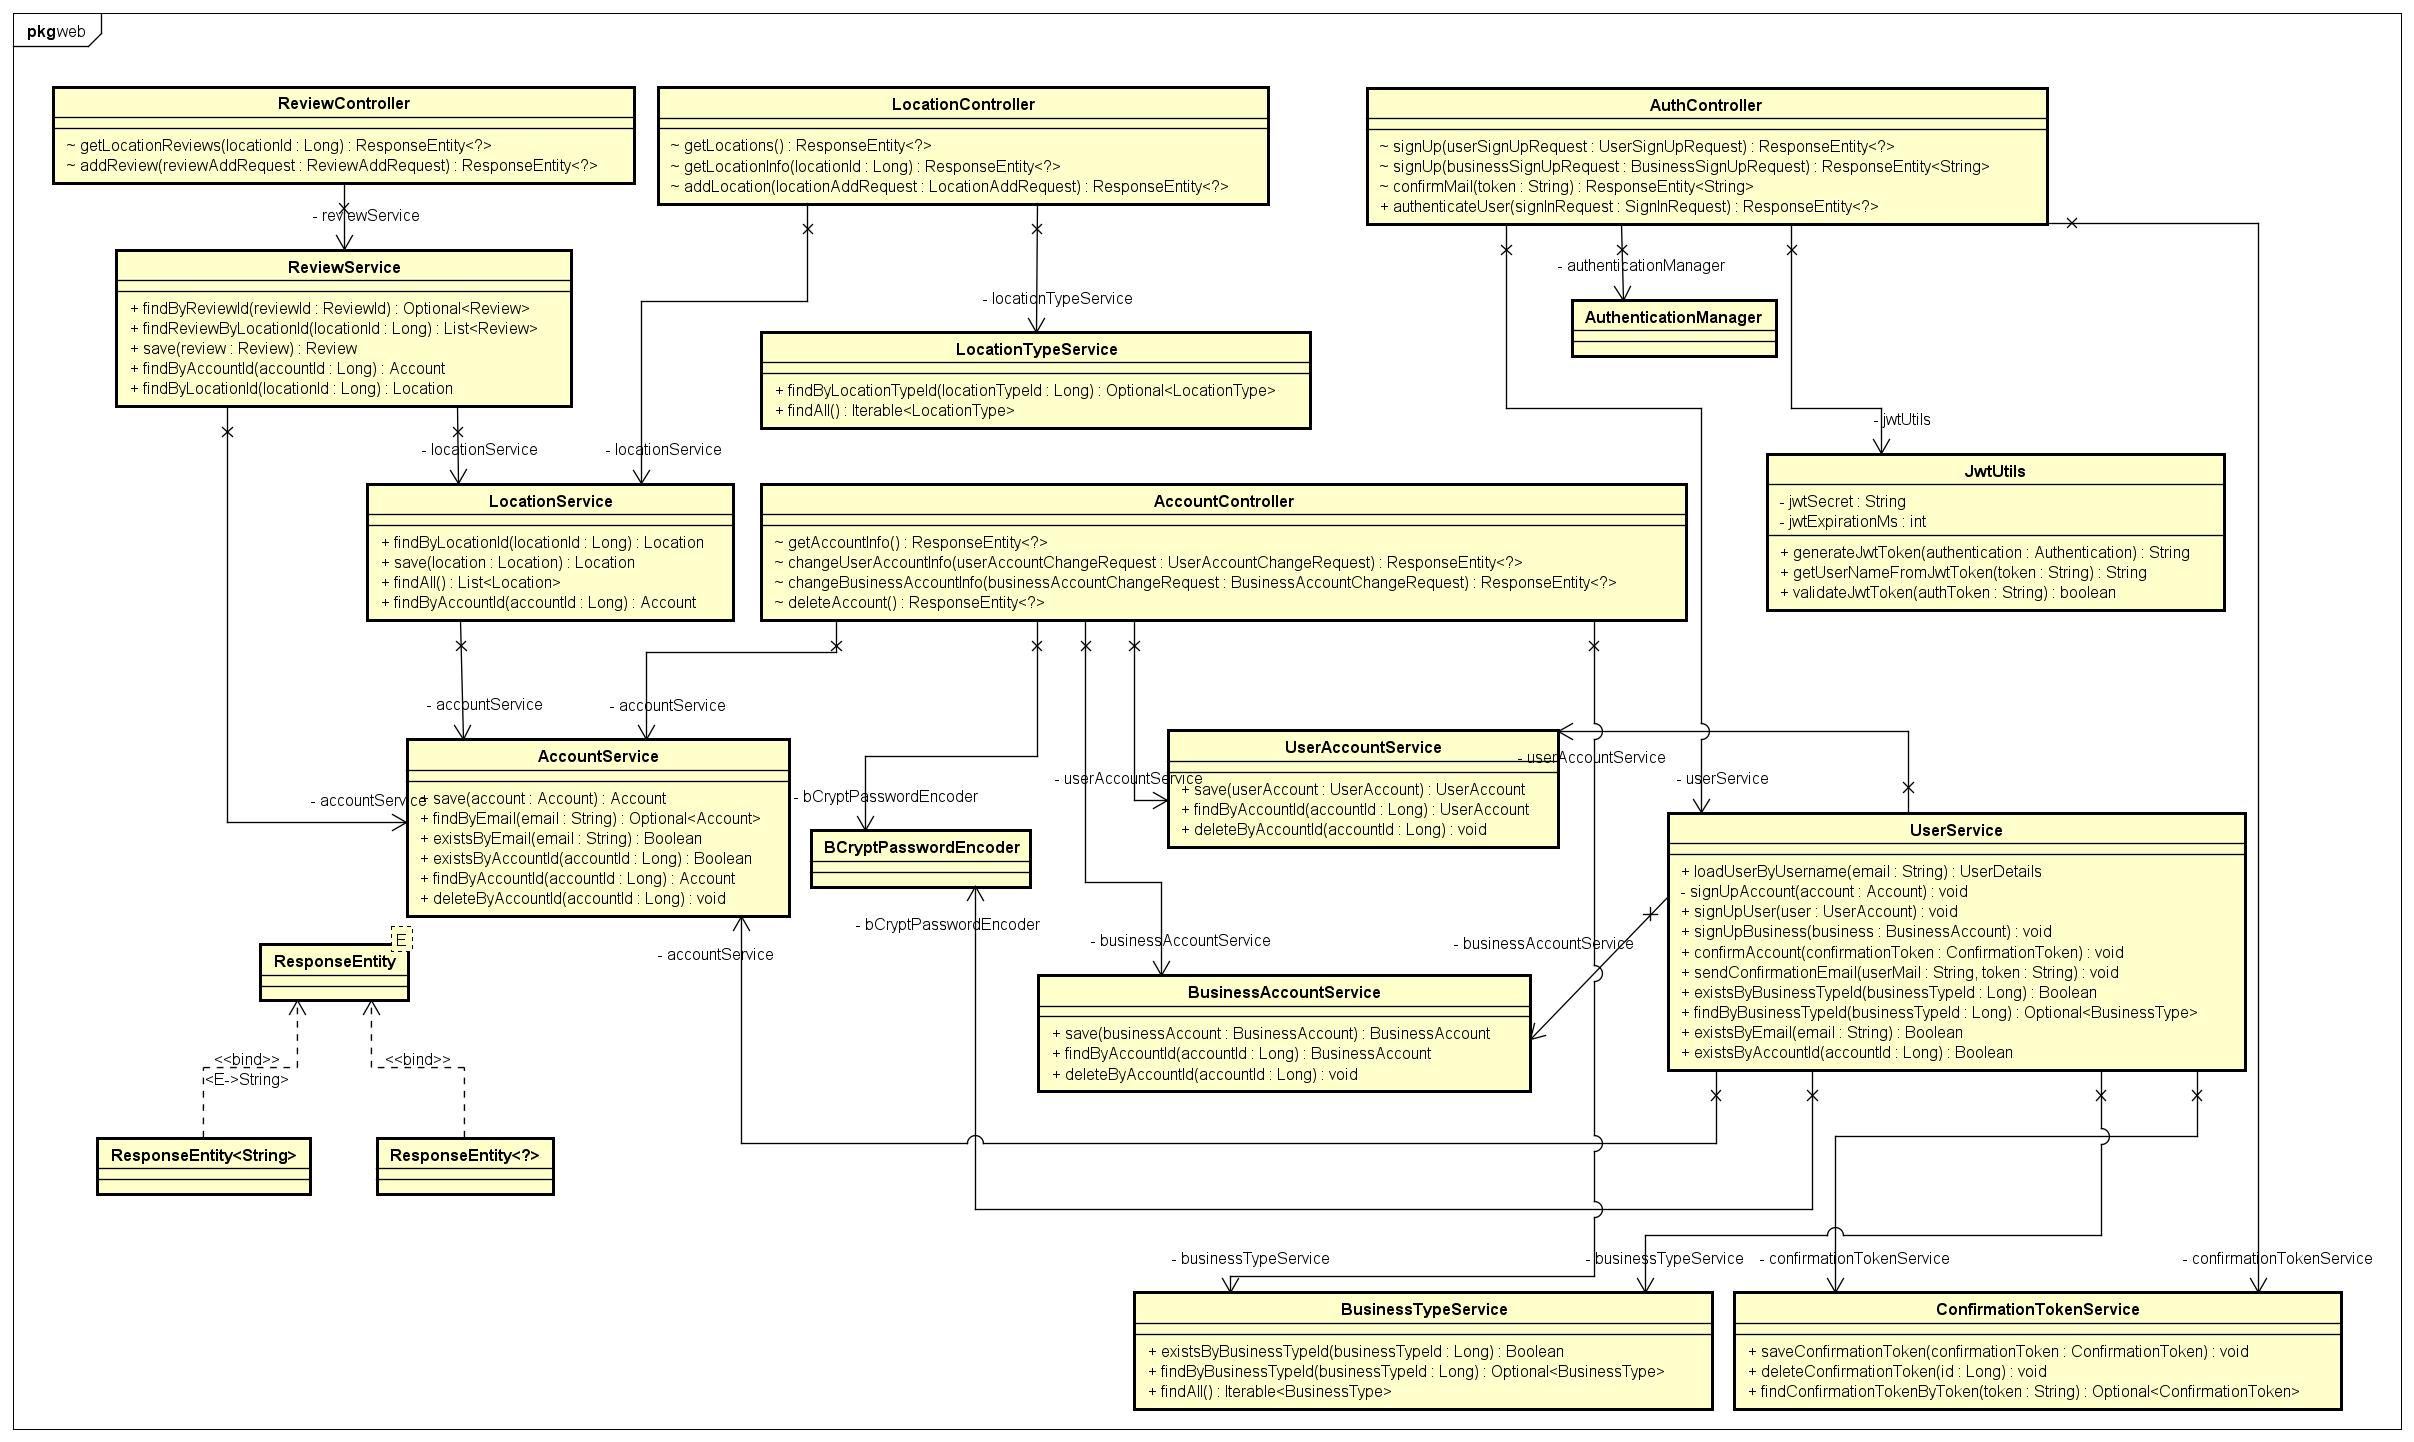
\includegraphics[width=\textwidth]{img/Dijagrami razreda/Controller_Class_Dijagram.jpg}
        	\centering
        	\caption{Controller class}
        	\label{fig:promjene}
        \end{figure}
        \begin{figure}[H]
        	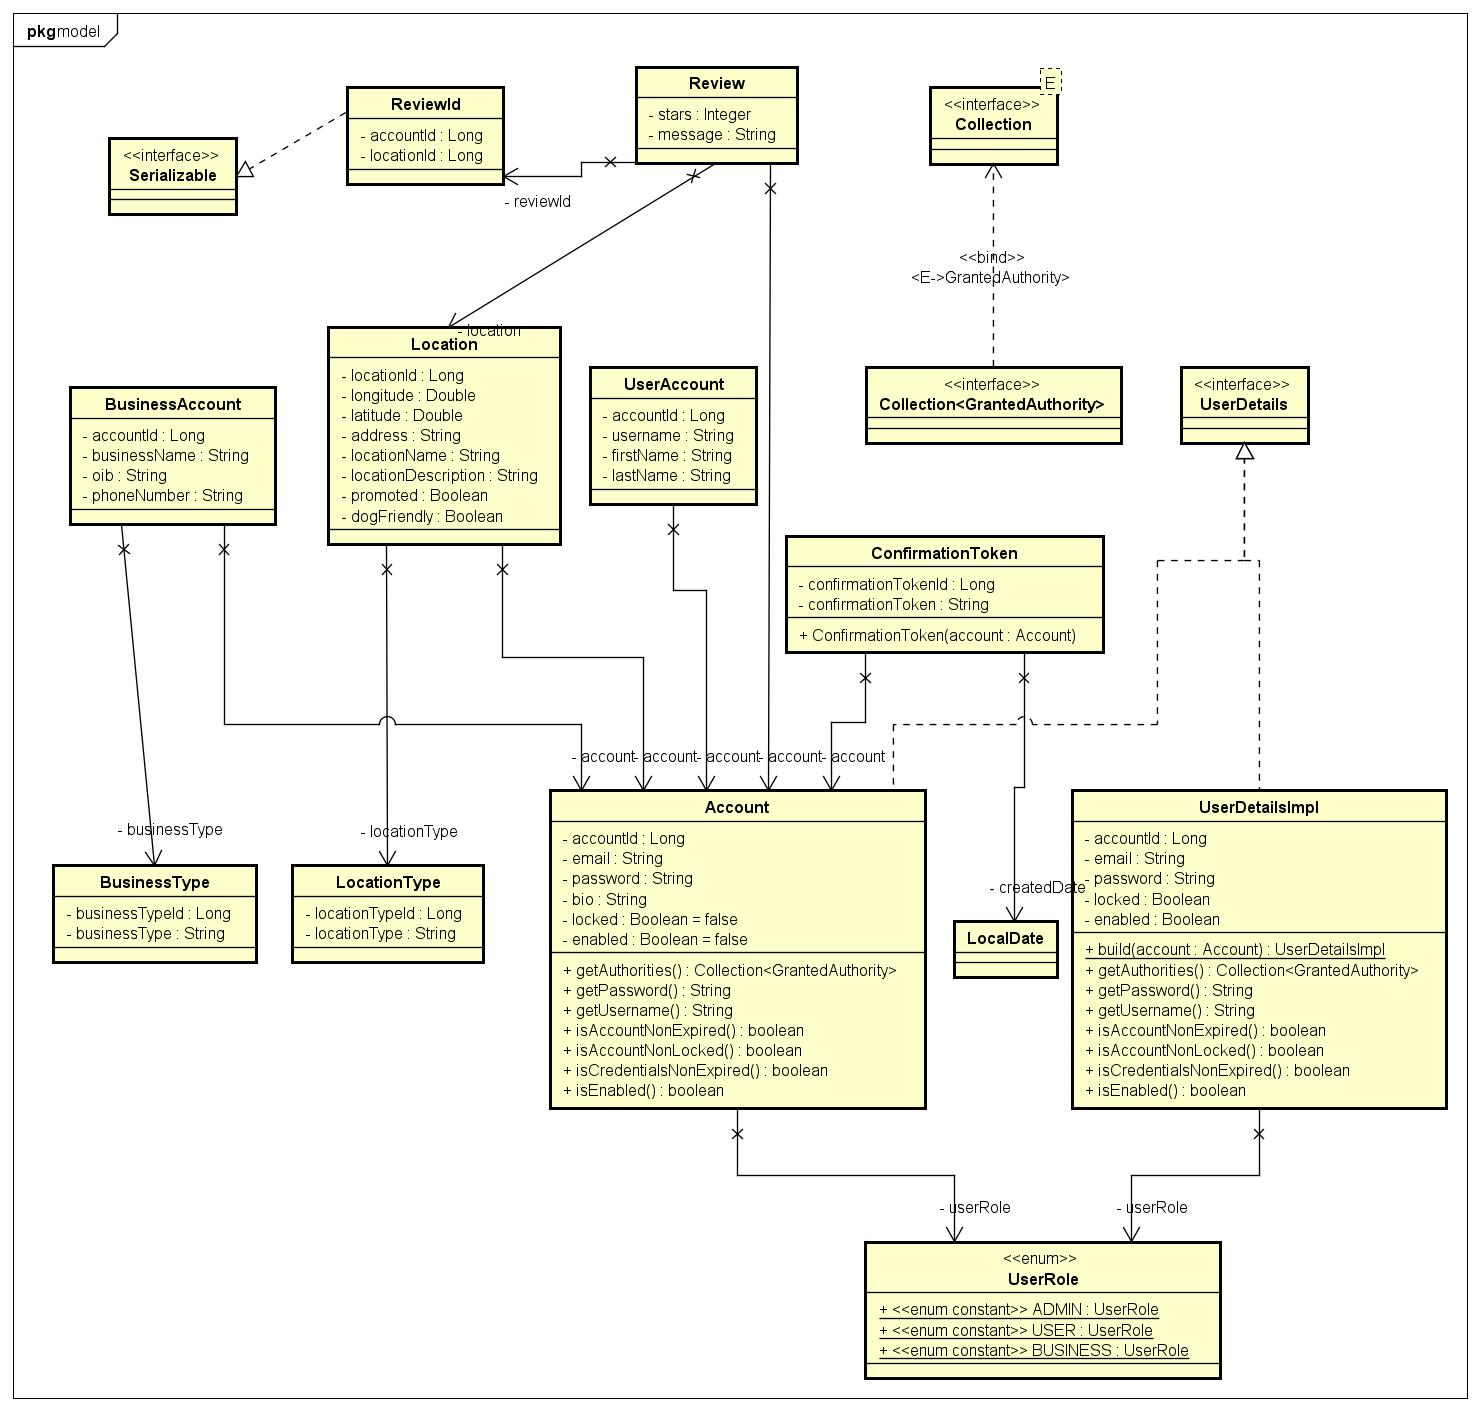
\includegraphics[width=\textwidth]{img/Dijagrami razreda/Model_Class_Dijagram.jpg}
        	\centering
        	\caption{Model class}
        	\label{fig:promjene}
        \end{figure}
        \begin{figure}[H]
        	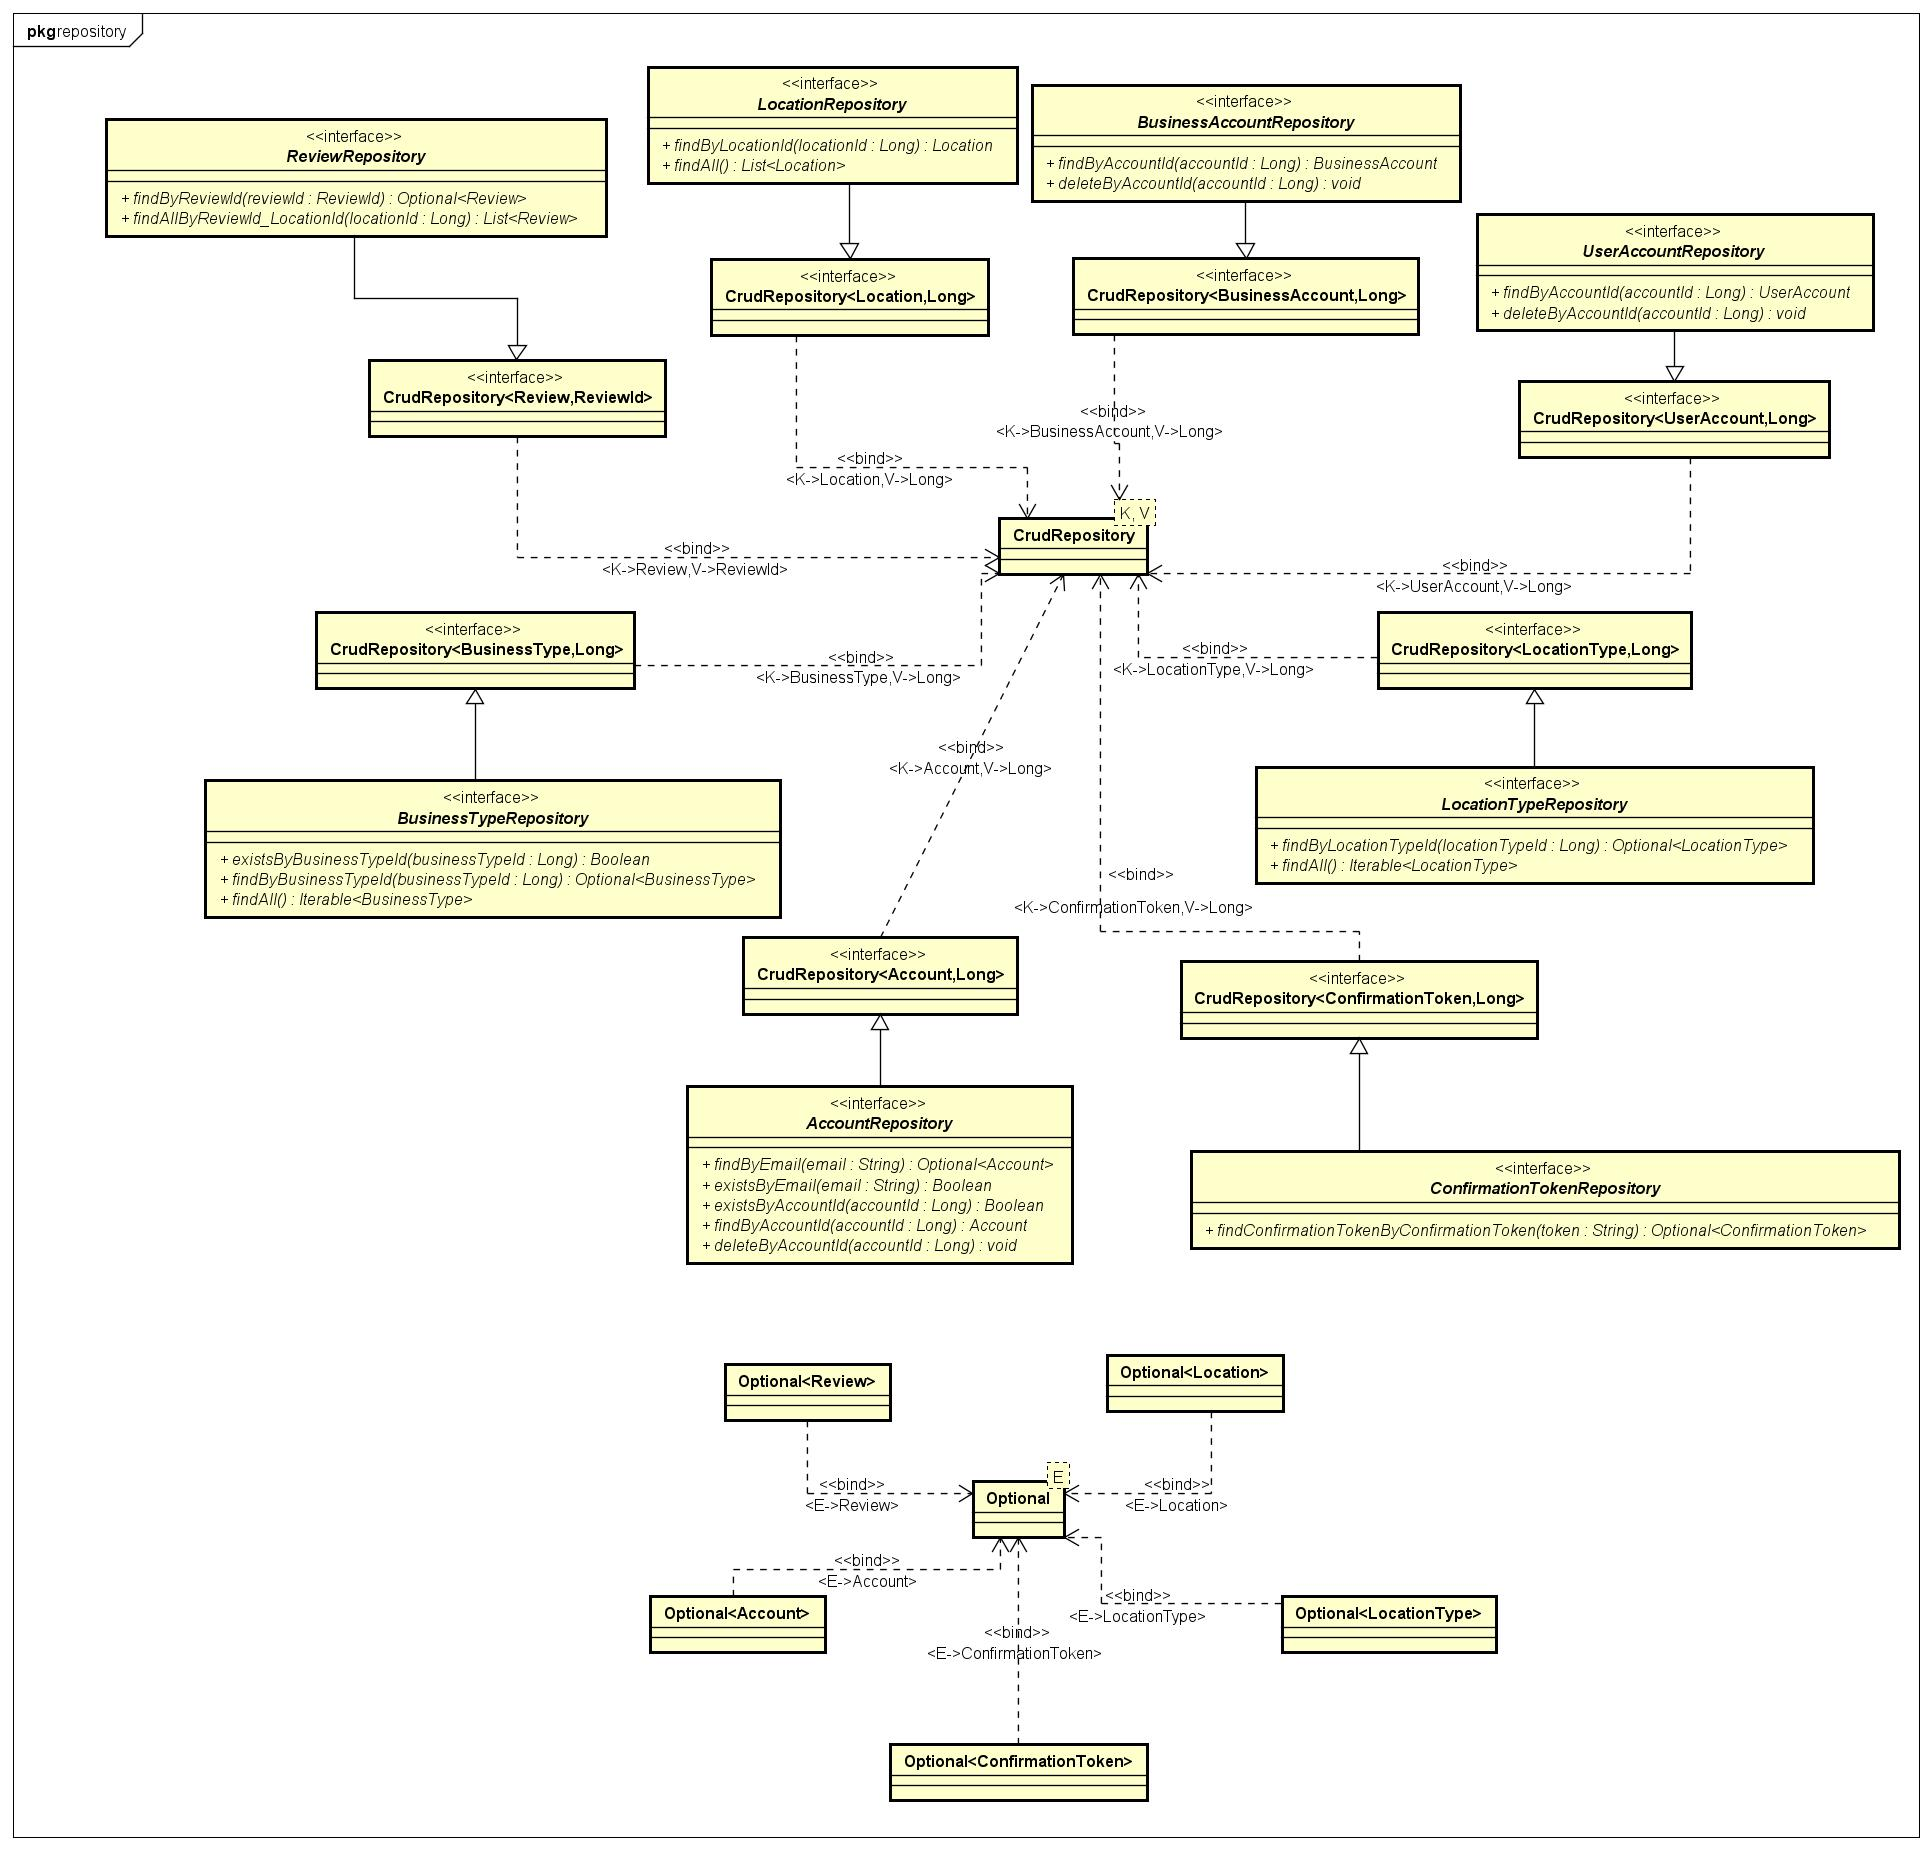
\includegraphics[width=\textwidth]{img/Dijagrami razreda/Repository_Class_Dijagram.jpg}
        	\centering
        	\caption{Repository class}
        	\label{fig:promjene}
        \end{figure}
        \begin{figure}[H]
        	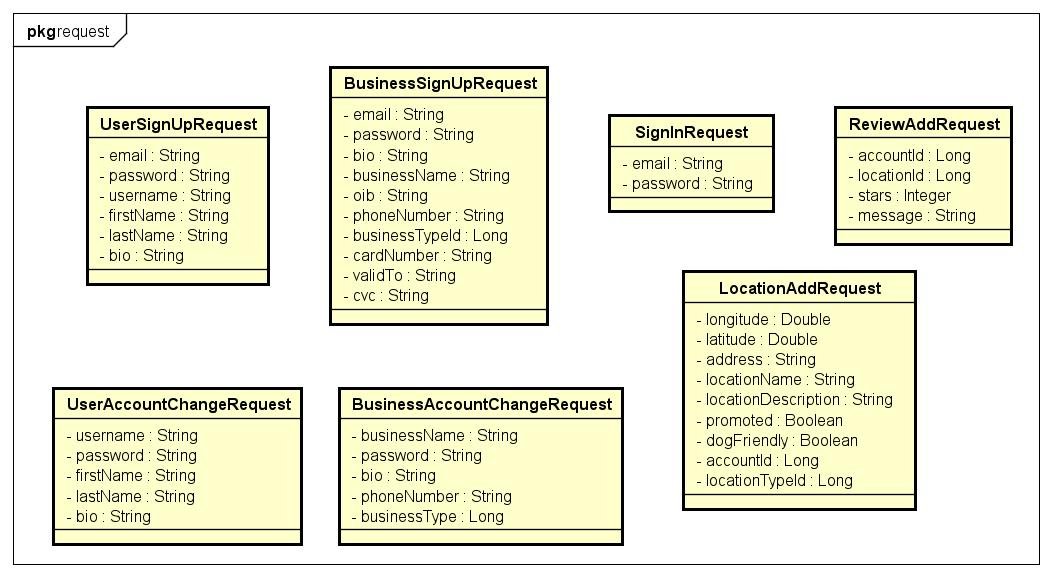
\includegraphics[width=\textwidth]{img/Dijagrami razreda/Request_Class_Dijagram.jpg}
        	\centering
        	\caption{Request class}
        	\label{fig:promjene}
        \end{figure}
        \begin{figure}[H]
        	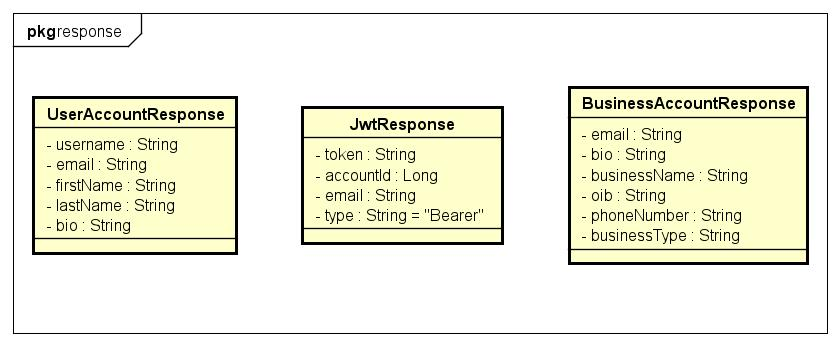
\includegraphics[width=\textwidth]{img/Dijagrami razreda/Response_Class_Dijagram.jpg}
        	\centering
        	\caption{Response class}
        	\label{fig:promjene}
        \end{figure}
        \begin{figure}[H]
        	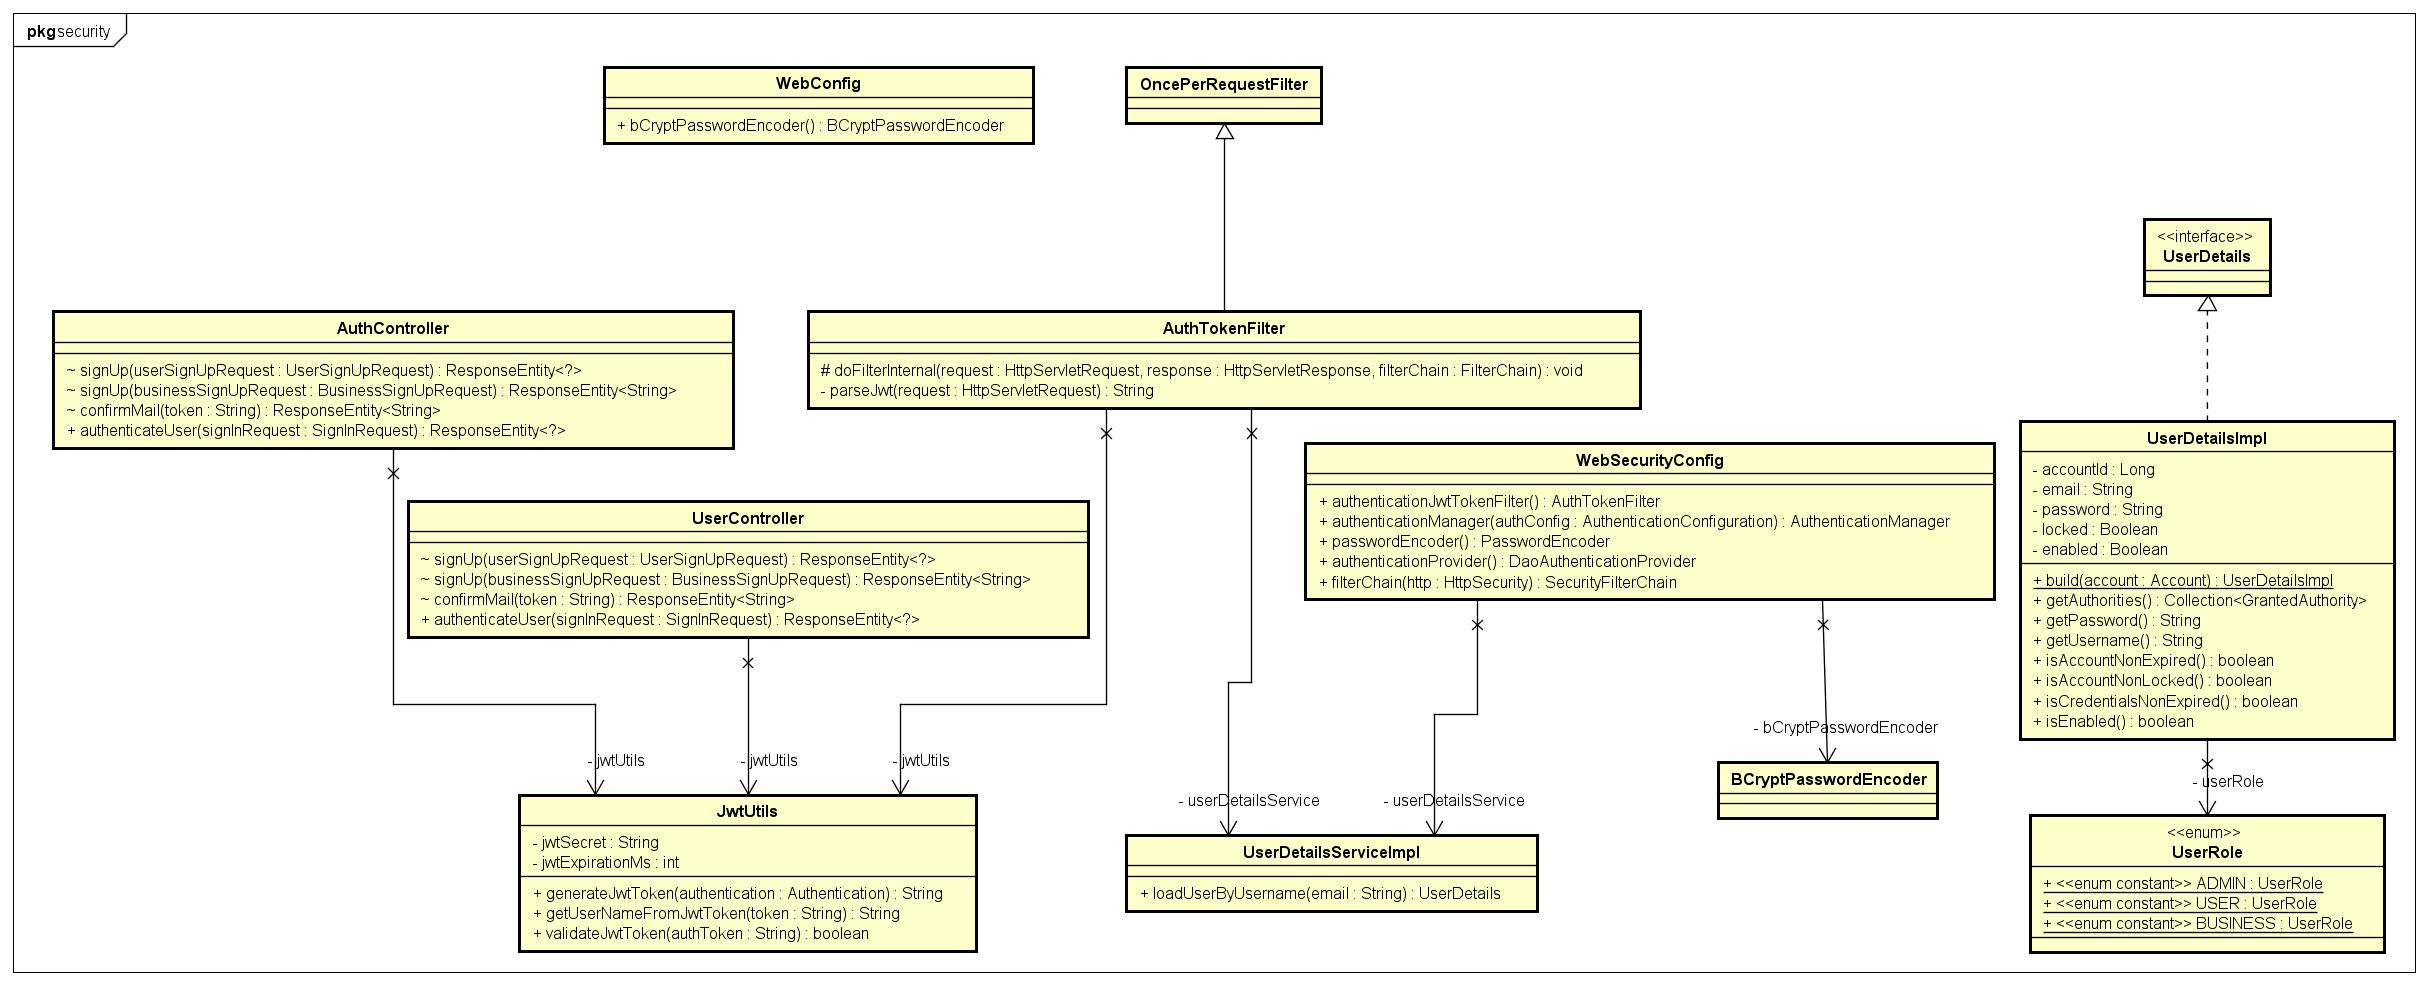
\includegraphics[width=\textwidth]{img/Dijagrami razreda/Security_Class_Dijagram.jpg}
        	\centering
        	\caption{Security class}
        	\label{fig:promjene}
        \end{figure}
        \begin{figure}[H]
        	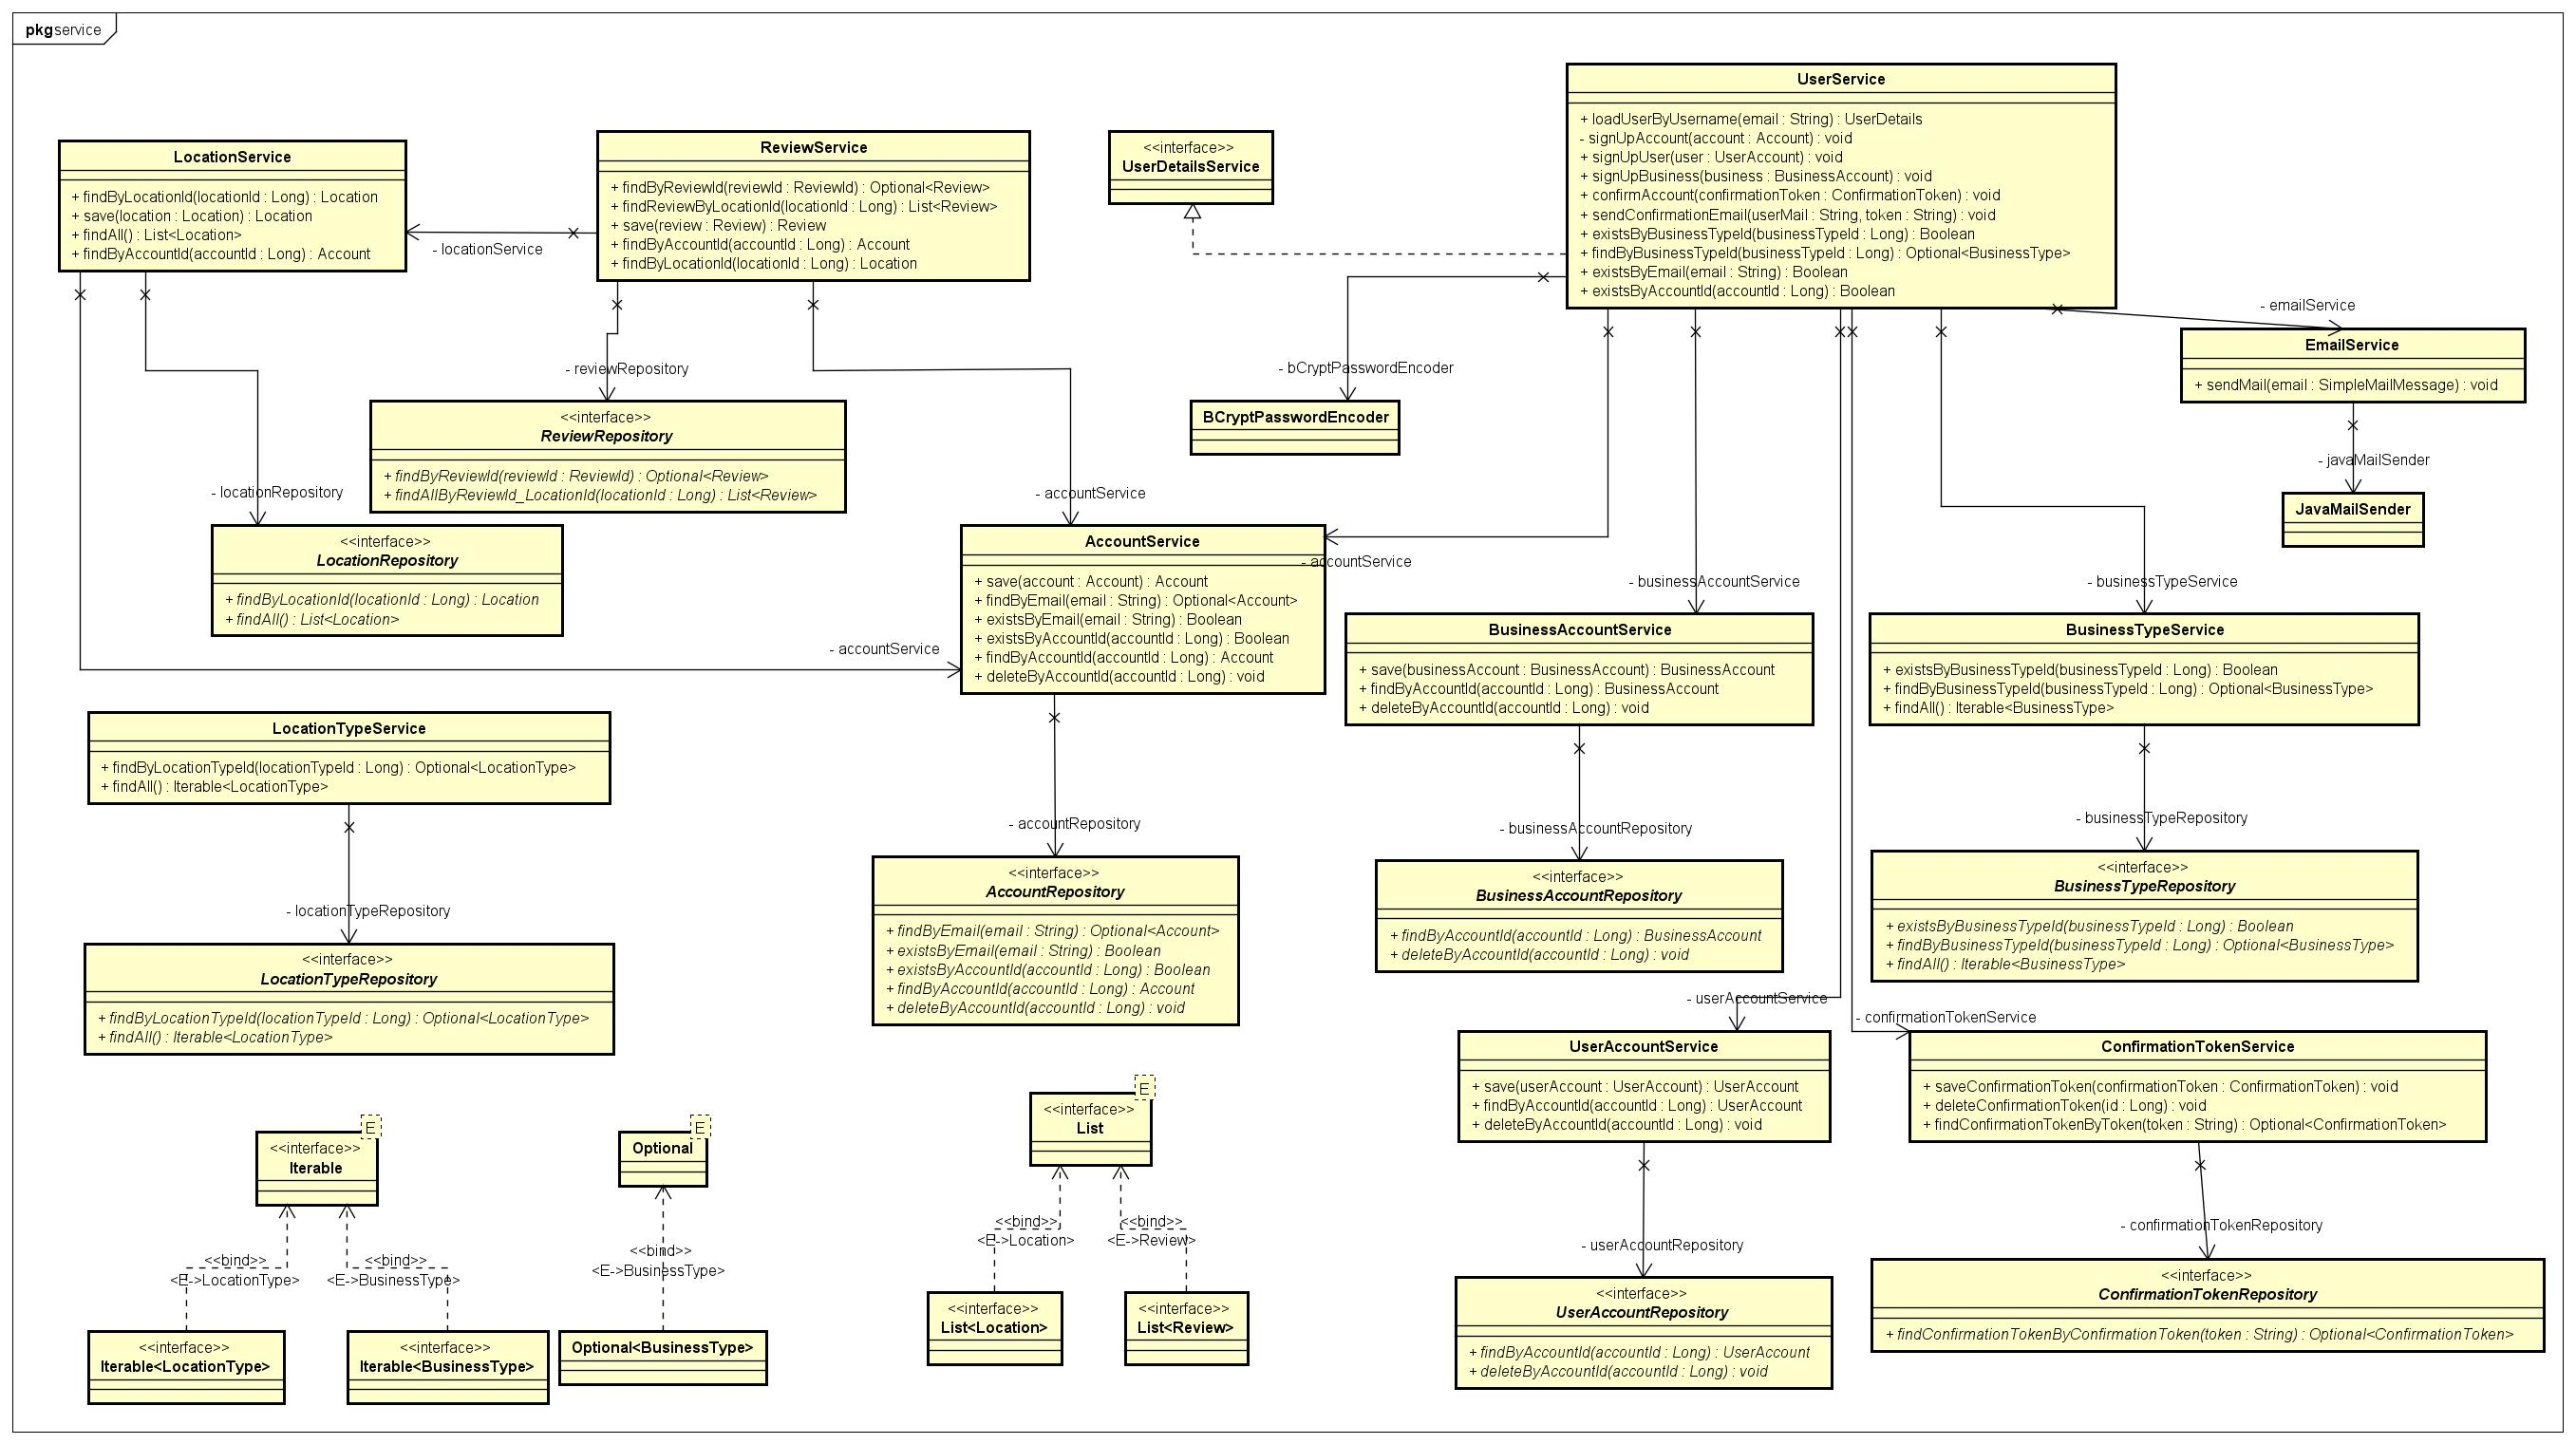
\includegraphics[width=\textwidth]{img/Dijagrami razreda/Service_Class_Dijagram.jpg}
        	\centering
        	\caption{Service class}
        	\label{fig:promjene}
        \end{figure}

        \eject
        \subsection{Dijagram razreda nakon završene aplikacije}
        \begin{figure}[H]
        	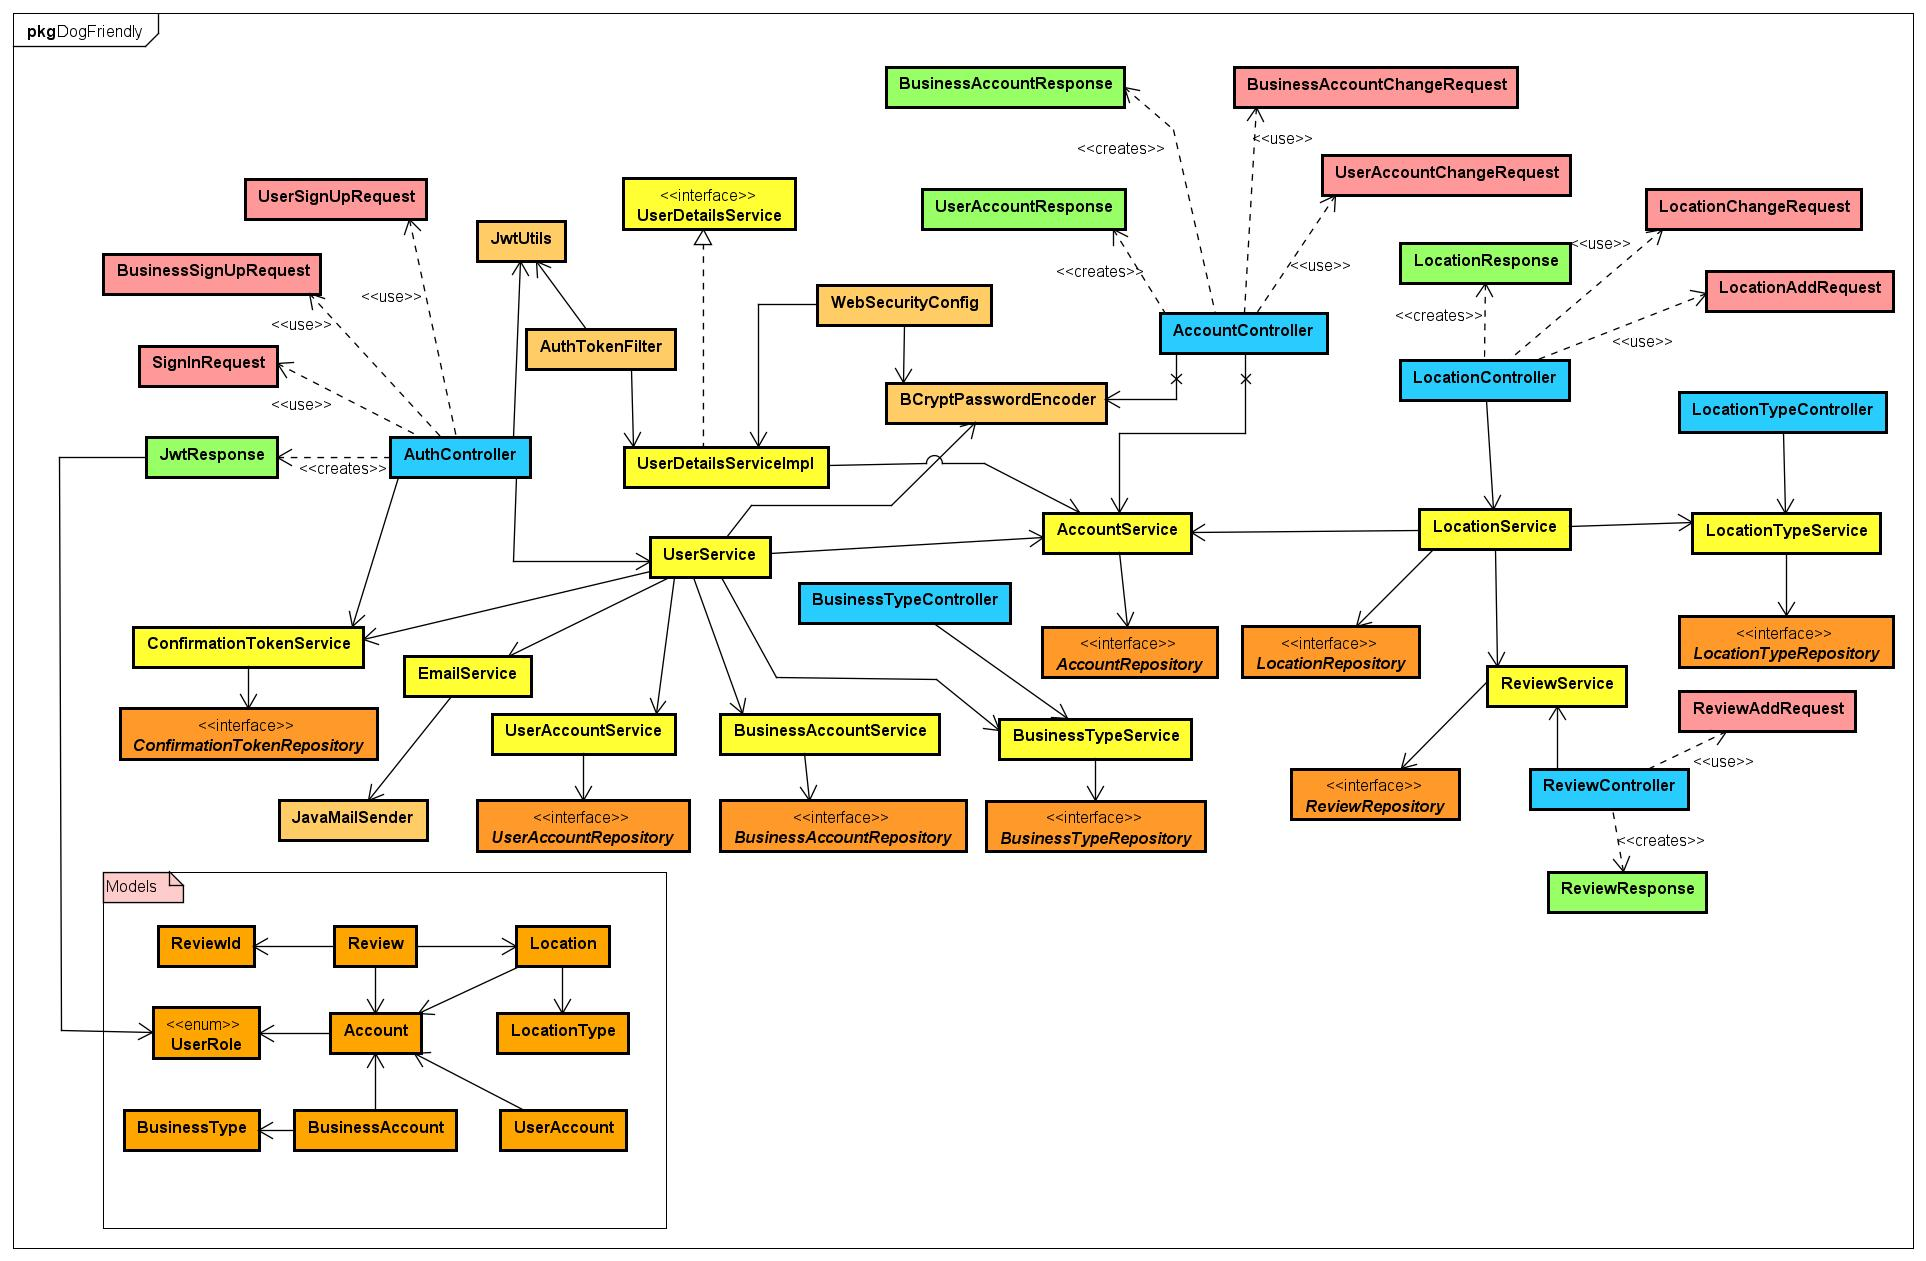
\includegraphics[width=\textwidth]{img/Dijagrami razreda/Class_Diagram.jpg}
        	\centering
        	\caption{Konceptualni dijagram razreda}
        	\label{fig:promjene}
        \end{figure}
    
    \eject
    \section{Dijagram stanja}

        Na slici je prikazan dijagram stanja za prijavljenog korisnika. Korisniku se otvara početna stranica s kartom. U gornjem desnom kutu je gumb koji ga vodi na njegov profil. Na svom profilu korisniku je omogućeno mijenjanje podataka profila ili brisanje računa. Također, sve lokacije koje je korisnik dodao su mu ponuđene na profilu da ih može mijenjati ili obrisati. Do podataka o lokaciji i pisanja recenzije može doći odabirom markera na karti ili pretraživanjem lokacije. Ako pretraživana lokacija ne postoji, korisniku se nudi opcija dodavanja lokacije.

        \begin{figure}[H]
        	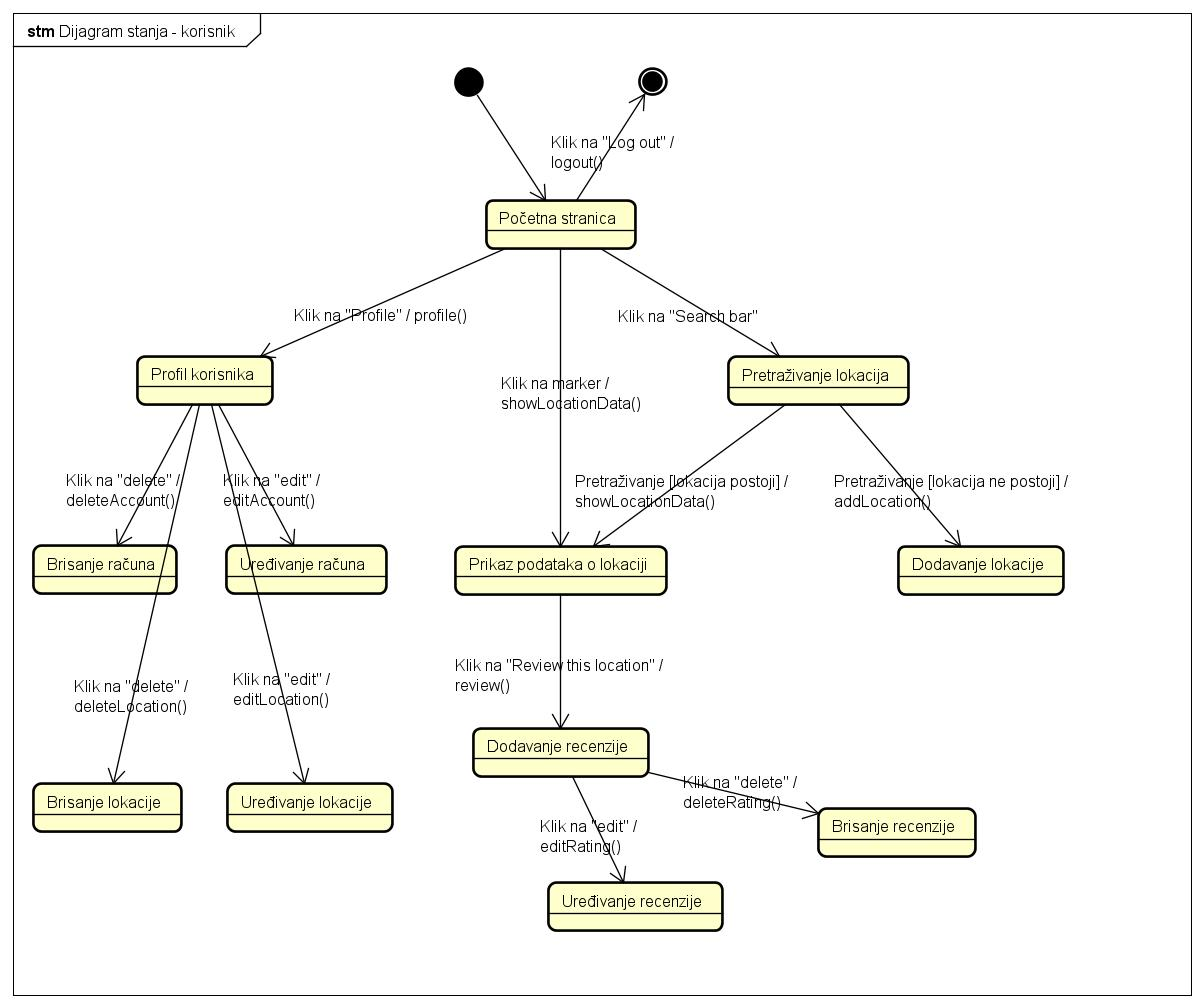
\includegraphics[width=\textwidth]{img/Dijagram stanja - korisnik.jpg}
        	\centering
        	\caption{Dijagram stanja}
        	\label{fig:promjene}
        \end{figure}

        \newpage 
    
    \section{Dijagram aktivnosti}
        Dijagram aktivnosti primjenjuje se za modeliranje upravljačkog i podatkovnog toka. U modeliranju toka upravljanja koristi se “pull” način djelovanja tj. svaki novi korak poduzima se nakon završenog prethodnog. Cilj je jednostavno i sažeto prikazati tok kontrole između pojedinih interakcija. Na dijagramu aktivnosti prikazan je proces pretraživanja i dodavanja lokacija registriranog korisnika. Korisnik, nakon prijave u sustav, pretražuje željenu lokaciju. U slučaju da lokacija već postoji u sustavu, prikazuju mu se podatci o odabranoj lokaciji, u suprotnom, registrirani korisnik ima mogućnost dodati novu vlastitu lokaciju. Ispravnim unosom podataka i ponovnim učitavanjem stranice lokacija postaje vidljiva na karti. 

        \begin{figure}[H]
        	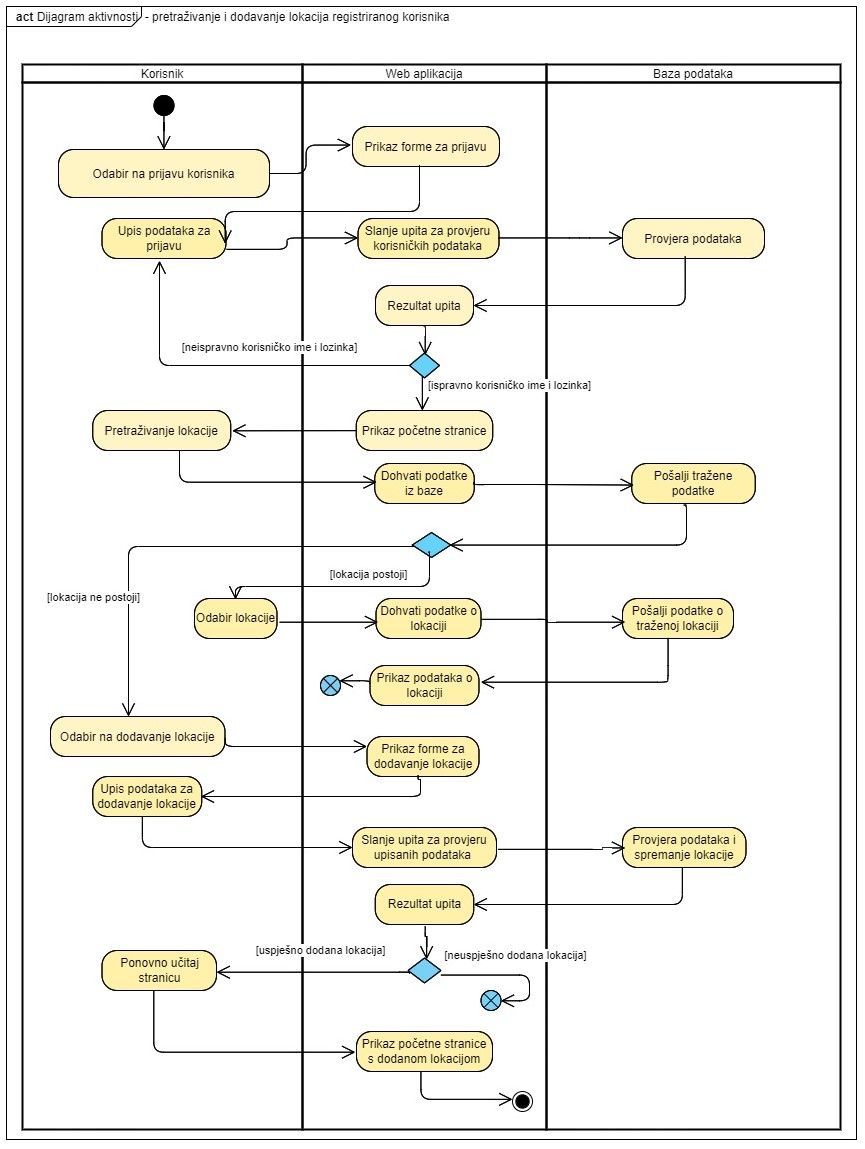
\includegraphics[width=\textwidth]{img/Dijagram aktivnosti.jpg}
        	\centering
        	\caption{Dijagram aktivnosti}
        	\label{fig:promjene}
        \end{figure}
    
    \section{Dijagram komponenti}

        Dijagram komponenti predstavlja specifikaciju arhitekture programske potpore i služi za vizualizaciju međuovisnosti i organizacije između implementacijskih komponenata. Sučeljem za dohvat HTML, CSS i JS datoteka se pristupa nginx komponenti koja poziva index.js. REST API komponenti se pristupa preko sučelja za dohvat JSON datoteka, a ona nam je potrebna za pristup bazi podataka.

        \begin{figure}[H]
        	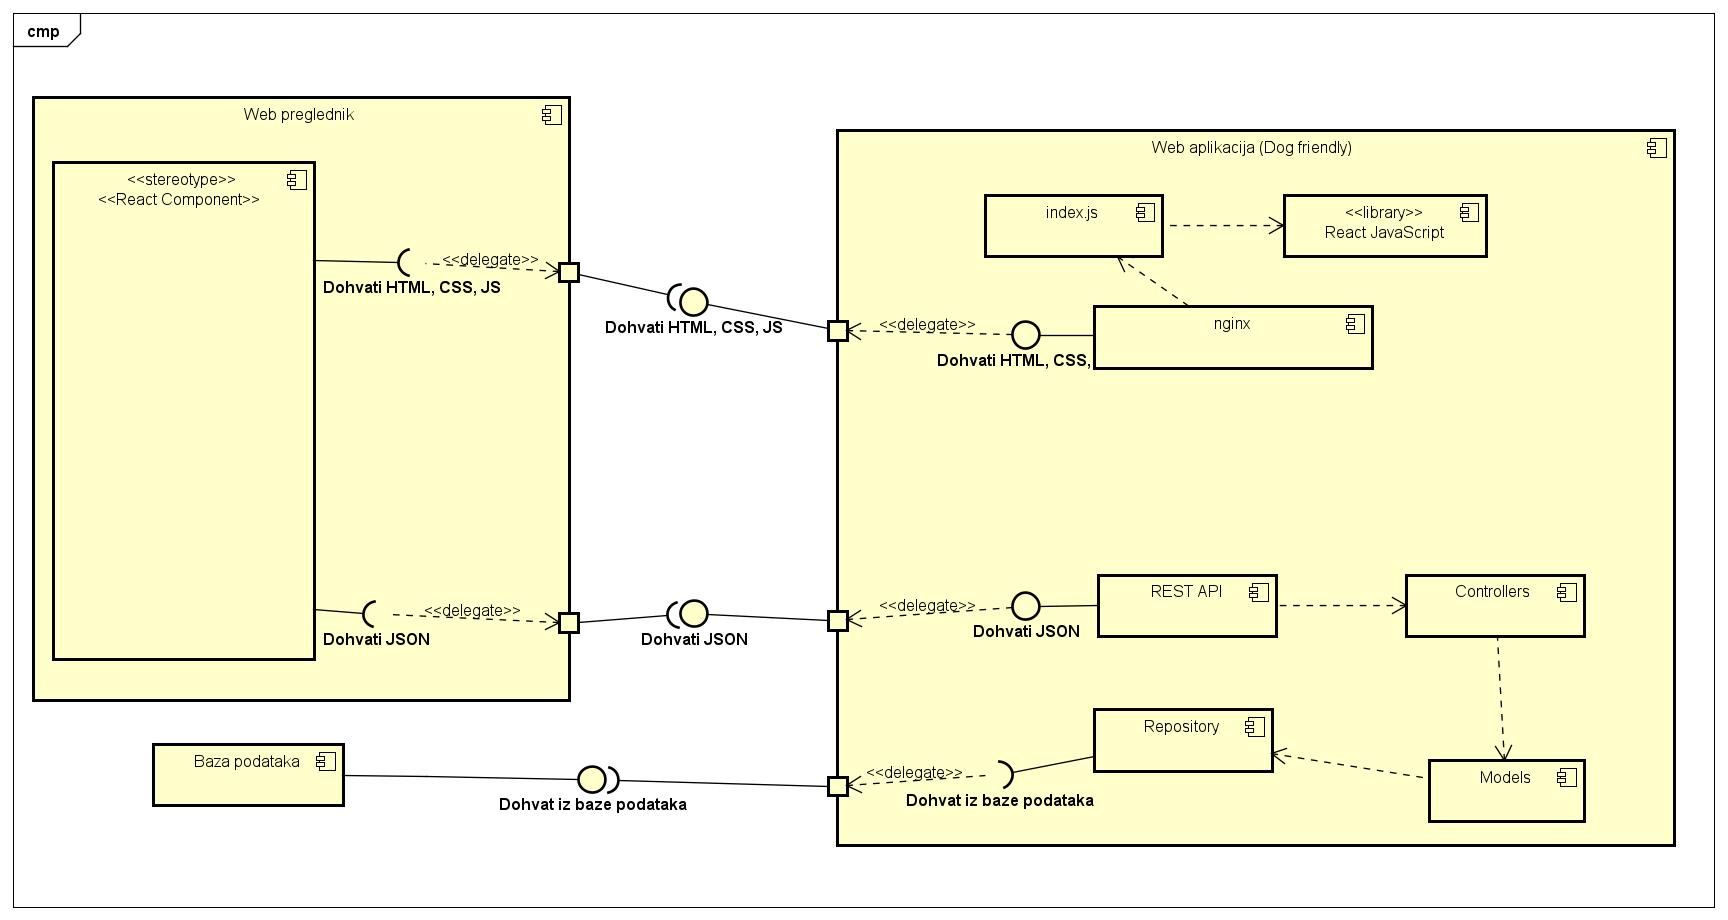
\includegraphics[width=\textwidth]{img/Dijagram komponenti.jpg}
        	\centering
        	\caption{Dijagram komponenti}
        	\label{fig:promjene}
        \end{figure}
    
		\chapter{Implementacija i korisničko sučelje}

    \section{Korištene tehnologije i alati}

    Koristili smo open-source sustav za upravljanje i pohranjivanje izvornog koda na platformi \textbf{GitLab}. \textit{( https://git-scm.com , https://gitlab.com )} \newline
    
    UML dijagrami izrađeni su uz pomoć \textbf{Astah Professional} aplikacije, a dijagrami baze podataka preko \textbf{ERDPlus}. \textit{( https://astah.net/products/astah-professional/ , https://erdplus.com/ )} \newline 
    
    Za komunikaciju s asistentom korišten je \textbf{Microsoft Teams}, a za međusobnu komunikaciju \textbf{WhatsApp}. Popis i podjela zadataka napravljena je na \textbf{Google Sheets}. \textit{( https://www.microsoft.com/hr-hr/microsoft-teams/group-chat-software/ , https://web.whatsapp.com/ , https://www.google.com/sheets/about/ )} \newline

    Za izradu dokumentacije primarno su korišteni \textbf{Overleaf} i \textbf{TeXstudio}. \textit{( https://www.overleaf.com , https://www.texstudio.org )} \newline
    
    Za pisanje frontend dijela aplikacije korištena je JavaScript biblioteka \textbf{React} te sintaksna ekstenzija JSX. Kod smo pisali u \textbf{Visual Studio Code-u}. Za kartu je korišten \textbf{Mapbox API}. \textit{( https://code.visualstudio.com , https://www.mapbox.com , https://www.npmjs.com , https://reactjs.org )} \newline
    
    Backend dio aplikacije pisan je u \textbf{Intellij IDEA} IDE-u u radnom okviru \textbf{Spring Boot} jezikom Java. \textit{( https://www.jetbrains.com/idea/ )} \newline

    Za deploy baze podataka (kao i aplikacije) korišten je \textbf{DigitalOcean}, a ista baza podataka korištena je i za testiranja. \textit{( https://www.digitalocean.com/ )}

    \section{Ispitivanje programskog rješenja}

    U nastavku ovog poglavlja biti će opisano ispitivanje implementiranih funkcionalnosti na razini komponenti te na razini cijelog sustava s prikazom odabranih ispitnih slučajeva.\newline
    
    U ispitivanju sustava korišten je radni okvir \textit{Selenium} te programsko sučelje \textit{Selenium WebDriver}. Metoda koja slijedi poziva se prije izvršavanja svakog testa.

    \begin{lstlisting}[language=Java,breaklines=true]
    @BeforeEach
	public void init() {
	   driver = new ChromeDriver();
	   System.setProperty("webdriver.chrome.driver", "C:\\Program Files (x86)\\Chrome Driver\\chromedriver.exe");
    
    driver.manage().timeouts().implicitlyWait(Duration.ofSeconds(10));
	   driver.get("http://dog-friendly.me/");
	}
    \end{lstlisting}

    \subsection{Ispitivanje komponenti}
    
    U prvom testu stvaramo objekt korisnika s već postojećim podatcima. Pozivamo funkciju koja se poziva prilikom pokušaja registracije. Test je uspješan ako test vrati vrijednost \textit{true} koja nam govori da korisnik s tom mail adresom već postoji.

    \begin{lstlisting}[language=Java,breaklines=true]
    @Test
    @Order(1)
    public void testCreateExistingUserException() {
        Account user = new Account(71l, "lm53309@fer.hr", "Husky123",
                "Novi dućan", UserRole.BUSINESS, false, false);

        accountService.existsByEmail(user.getEmail());

        assertEquals(true, accountService.existsByEmail(user.getEmail()));
    }
    \end{lstlisting}

    \eject
    Drugi test provjerava funkciju promjene podataka lokacije. Želimo promijeniti samo jedan podatak (u ovom slučaju opis) dok ostali podatci moraju ostati isti. Test je Uspješan ako je objekt nakon promjene jednak spremljenoj lokaciji s novim podatkom.

    \begin{lstlisting}[language=Java, breaklines=true]
    @Test
    @Order(2)
    public void testLocationChange() {
        LocationChangeRequest locationChangeRequest = new LocationChangeRequest(2l, null,
                null, "Fakultet elektrotehnike i računarstva", null, null);
        LocationResponse locationResponse = locationService.getByLocationId(locationChangeRequest.getLocationId());
        Location location = new Location(
                locationResponse.getLocationId(),
                locationResponse.getLongitude(),
                locationResponse.getLatitude(),
                locationResponse.getAddress(),
                locationChangeRequest.getLocationName() != null ? locationChangeRequest.getLocationName() : locationResponse.getLocationName(),
                locationChangeRequest.getLocationDescription() != null ? locationChangeRequest.getLocationDescription() : locationResponse.getLocationDescription(),
                locationChangeRequest.getPromoted() != null ? locationChangeRequest.getPromoted() : locationResponse.getPromoted(),
                locationChangeRequest.getDogFriendly() != null ? locationChangeRequest.getDogFriendly() : locationResponse.getDogFriendly(),
                accountService.findByAccountId(71l),
                locationTypeService.findByLocationTypeId(locationChangeRequest.getLocationTypeId() != null ? locationChangeRequest.getLocationTypeId() : locationResponse.getLocationTypeId()).orElse(null)
        );

        locationService.save(location);

        assertEquals(location, locationService.save(location));
    }
    \end{lstlisting}

    \eject
    Treći test radi provjeru funkcije za pretraživanje. Navodimo string lokacije koja postoji u sustavu. Test je uspješan ako je lokacija nađena funkcijom jednaka stringu.

    \begin{lstlisting}[language=Java, breaklines=true]
    @Test
    @Order(3)
    public void testSearchLocation() {
        String description = "808";
        List<LocationResponse> locations = locationService.search(description);
        LocationResponse location = locations.get(0);

        assertEquals("808", location.getLocationName());
    }
    \end{lstlisting}

    Četvrtim testom pokušavamo dohvatiti srednju vrijednost recenzije za lokaciju određenu s \textit{locationId}. Test je uspješan ako je dohvaćena vrijednost jednaka očekivanoj.

    \begin{lstlisting}[language=Java, breaklines=true]
    @Test
    @Order(4)
    public void testReviewAverage() {
        Long locationId = 2l;
        reviewService.getAverageForLocation(locationId);
        double avrg = (double) 13/3;

        assertEquals(Double.valueOf(avrg), reviewService.getAverageForLocation(locationId));
    }
    \end{lstlisting}

    Peti test provjerava funkciju za autentifikaciju korisnika. Korisnik se pokušava ulogirati na račun, ali s pogrešnom lozinkom. Ovaj test je uspješan ako kao odgovor dobijemo HttpStatus.BADREQUEST.

    \begin{lstlisting}[language=Java, breaklines=true]
    @Test
    @Order(5)
    public void testIncorrectPassword() {
        String email = "lm53309@fer.hr";
        String password = "provala";

        Authentication authentication;
        ResponseEntity responseEntity = new ResponseEntity(HttpStatus.OK);

        try {
            authentication = authenticationManager.authenticate(
                    new UsernamePasswordAuthenticationToken(email, password));
        } catch(BadCredentialsException e) {
            responseEntity = new ResponseEntity<>(HttpStatus.BAD_REQUEST);
        }

        assertEquals(HttpStatus.BAD_REQUEST, responseEntity.getStatusCode());
    }
    \end{lstlisting}

    U posljednjem testu provjeravamo povezanost lokacije s korisnikom koji ju je kreirao. Korisnik pokušava promijeniti lokaciju koju on nije kreirao. Prilikom promjene prvo se provjerava ima li korisnik ovlasti za odabranu akciju. Test je uspješan ako kao odgovor dobijemo da korisnik nema dozvolu za promjenu (HttpStatus.UNAUTHORIZED).

    \begin{lstlisting}[language=Java, breaklines=true]
    @Test
    @Order(6)
    public void testUnauthorizedLocationChange() {
        Long currentlyLoggedInAccountId = 71l;
        Long locationId = 196l;
        LocationResponse locationResponse = locationService.getByLocationId(locationId);
        ResponseEntity responseEntity = new ResponseEntity(HttpStatus.OK);

        if(locationResponse.getAccountId() != currentlyLoggedInAccountId)
            responseEntity = new ResponseEntity<>(HttpStatus.UNAUTHORIZED);

        assertEquals(HttpStatus.UNAUTHORIZED, responseEntity.getStatusCode());
    }
    \end{lstlisting}

    \eject
    \textbf{Svi ispitani testovi su bili uspješni}

    \begin{figure}[H]
        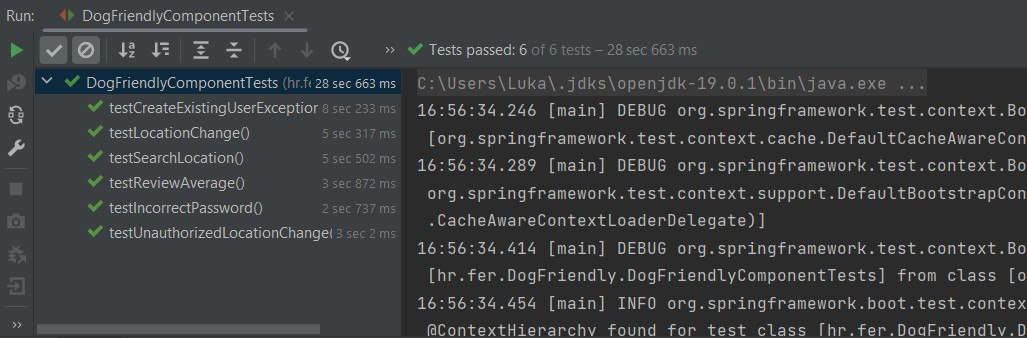
\includegraphics[width=\textwidth]{img/Ispitivanje komponentni.jpg}
        \centering
        \caption{Rezultati testova ispitivanja komponenti}
    \end{figure}

    \subsection{Ispitivanje sustava}

    Prvi test ispituje uspješnu prijavu registriranog korisnika u sustav. Test je uspješan ako Selenium sustav dođe do \textit{homepage-a}, tj. URL Web preglednika više ne sadrži \textit{/login}.

    \begin{lstlisting}[language=Java,breaklines=true]
    @Test
    @Order(1)
    void testUserLoginGoodCreds() {
		      driver.findElement(By.id("account-info")).click();
		      driver.findElement(By.id("login")).click();

		      WebElement element = driver.findElement(By.id("inputEmail"));
		      element.sendKeys("mario.hosnjak009@gmail.com");

		      element = driver.findElement(By.id("inputPassword"));
		      element.sendKeys("lozinka");

		      driver.findElement(By.className("button")).click();

		      try {
			     Thread.sleep(1000);
		      } catch (Exception e) {
			     e.printStackTrace();
		      }

		      String redirectedURL = driver.getCurrentUrl();
		      boolean result = !(redirectedURL.contains("login"));

		      assertTrue(result);
	}
    \end{lstlisting}

    Drugi će test isprovocirati grešku u sustavu tako što će se sustav Selenium pokušati prijaviti s pogrešnim emailom i/ili lozinkom. Test će biti uspješan ako se pojavi poruka "Pogrešan e-mail ili lozinka".

    \begin{lstlisting}[language=Java,breaklines=true]
    @Test
	@Order(2)
	void testUserLoginBadCreds() {
		driver.findElement(By.id("account-info")).click();
		driver.findElement(By.id("login")).click();

		WebElement element = driver.findElement(By.id("inputEmail"));
		element.sendKeys("krivi.email@gmail.com");

		element = driver.findElement(By.id("inputPassword"));
		element.sendKeys("krivalozinka");

		driver.findElement(By.className("button")).click();

		try {
			Thread.sleep(1000);
		} catch (Exception e) {
			e.printStackTrace();
		}

		String errorMsg = driver.findElement(By.cssSelector("div p")).getAttribute("innerHTML");

		assertTrue(errorMsg.contains("Pogrešan e-mail ili lozinka"));
	}
    \end{lstlisting}
    
    Treći test ispituje uspješno uređivanje podataka profila registriranog korisnika. Test se smatra uspješnim ako sustav Selenium uspije pročitati nove podatke sa stranice korisničkog profila.

    \begin{lstlisting}[language=Java,breaklines=true]
    @Test
    @Order(3)
    void testEditUserInfo() {
    		testUserLoginGoodCreds();
    		driver.findElement(By.id("account-info")).click();
    		driver.findElement(By.id("profileInfo")).click();
		driver.findElement(By.cssSelector("#editInfo > path:nth-child(2)")).click();

    		WebElement element = driver.findElement(By.id("editUsername"));
    		element.clear();
    		element.sendKeys("AutomatedTestUsername");
    
    		element = driver.findElement(By.id("editPassword"));
    		element.sendKeys("lozinka");

    		element = driver.findElement(By.id("editBio"));
    		element.clear();
    		element.sendKeys("AutomatedTestBio");
    
    		driver.findElement(By.id("saveChanges")).click();

		      try {
			     Thread.sleep(2000);
		      } catch (Exception e) {
			     e.printStackTrace();
		      }

		      String resElement1 = driver.findElement(By.name("username")).getAttribute("innerHTML");
		      String resElement2 = driver.findElement(By.name("bio")).getAttribute("innerHTML");

		      assertTrue(resElement1.contains("AutomatedTestUsername") && resElement2.contains("AutomatedTestBio"));
    }
    \end{lstlisting}
    
    Četvrti test ispituje uspješno dodavanje recenzije na neku lokaciju. Test se smatra uspješnim ako sustav Selenium uspije pročitati novu recenziju.

    \begin{lstlisting}[language=Java,breaklines=true]
    @Test
    @Order(4)
    void testAddReview() {
		      testUserLoginGoodCreds();
    		driver.findElement(By.id("search")).click();
    
    		WebElement element = driver.findElement(By.id("search"));
    		element.sendKeys("Proba");
    
    		driver.findElement(By.id("0")).click();
    		driver.findElement(By.className("review-location-btn")).click();
    		driver.findElement(By.cssSelector("span:nth-child(4)")).click();
    
    		element = driver.findElement(By.cssSelector("textarea"));
    		element.sendKeys("Automated Test Review");
    
    		driver.findElement(By.id("submitReview")).click();
    
		      String reviewRes = driver.findElement(By.name("reviewText")).getAttribute("innerHTML");

		      assertTrue(reviewRes.contains("Automated Test Review"));
    }
    \end{lstlisting}

    \textbf{Sve ispitane funkcionalnosti su uspješno ispitane te svi testovi prolaze.}

    \begin{figure}[H]
        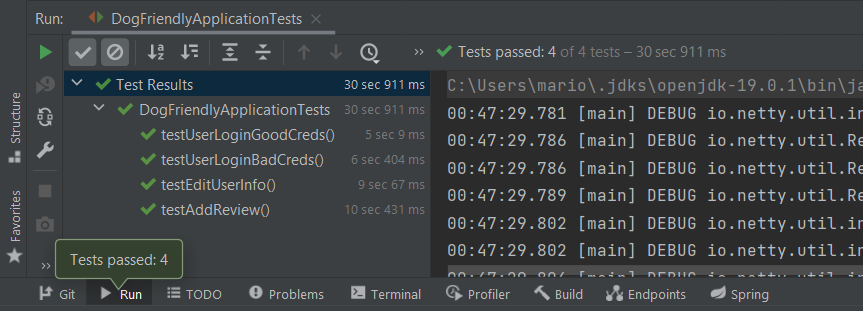
\includegraphics[width=\textwidth]{img/TestSuccess4.png}
        \centering
        \caption{Rezultati testova ispitivanja sustava}
    \end{figure}

    \eject
    \section{Dijagram razmještaja}

    Dijagram razmještaja prikazuje odnos programskih i sklopovskih dijelova te opisuje topologiju sustava. Klijent, koristeći HTTP protokol, preko klijentskog računala pristupa poslužiteljskom računalu. Poslužitelj koristi radni okvir Node.js preko kojeg se dohvaća stranica, Tomcat koji sadrži aplikaciju i funkcionalnosti te PostgreSql s bazom podataka.

    \begin{figure}[H]
        	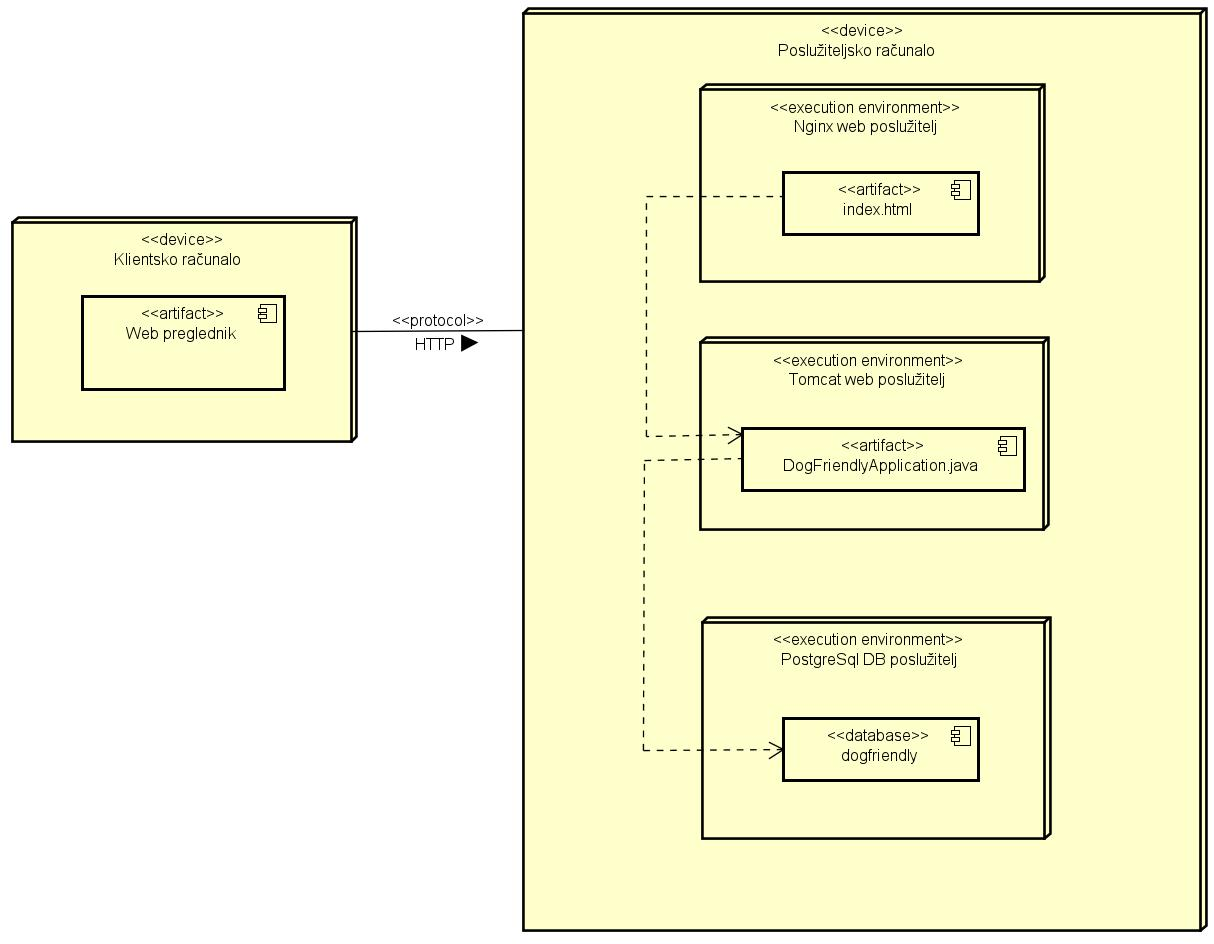
\includegraphics[width=\textwidth]{img/Dijagram_razmjestaja.jpg}
        	\centering
        	\caption{Dijagram razmještaja}
        	\label{fig:promjene}
        \end{figure}

    \eject
    \section{Upute za puštanje u pogon}

    Preduvjet za slijeđenje sljedećih uputa je instalirana instanca Ubuntu 22.04 operacijskog sustava na poslužitelju. Koraci u ovim uputama će gotovo sigurno raditi bez modifikacija na ostalim modernim inačicama Ubuntu operacijskog sustava, a uz manje modifikacije i na ostalim Linux operacijskim sustavima.

    \subsection{Konfiguracija baze podataka}

    Instalacija i pokretanje postgresql servisa
    \begin{lstlisting}[language=bash]
      sudo apt update
      sudo apt install postgresql postgresql-contrib
      sudo systemctl start postgresql.service
    \end{lstlisting}

    Zatim je potrebno konfigurirati vatrozid
    \begin{lstlisting}[language=bash]
      sudo ufw allow 5432
    \end{lstlisting}

    Sada se na sustav za upravljanje bazom podataka moguće spojiti pomoću alata PgAdmin. Potrebno je kliknuti na gumb "Add New Server" i zatim popuniti polja prikazana na slici.

    \begin{figure}[H]
    \centering
    \begin{subfigure}{.5\textwidth}
      \centering
      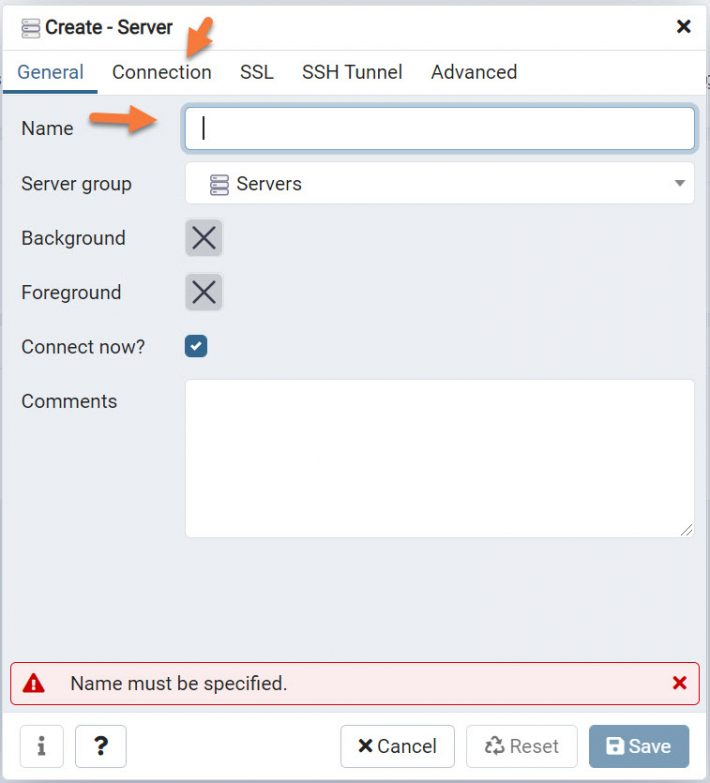
\includegraphics[width=0.9\linewidth]{img/2-1-710x783.jpg}
      \label{fig:sub1}
    \end{subfigure}%
    \begin{subfigure}{.5\textwidth}
      \centering
      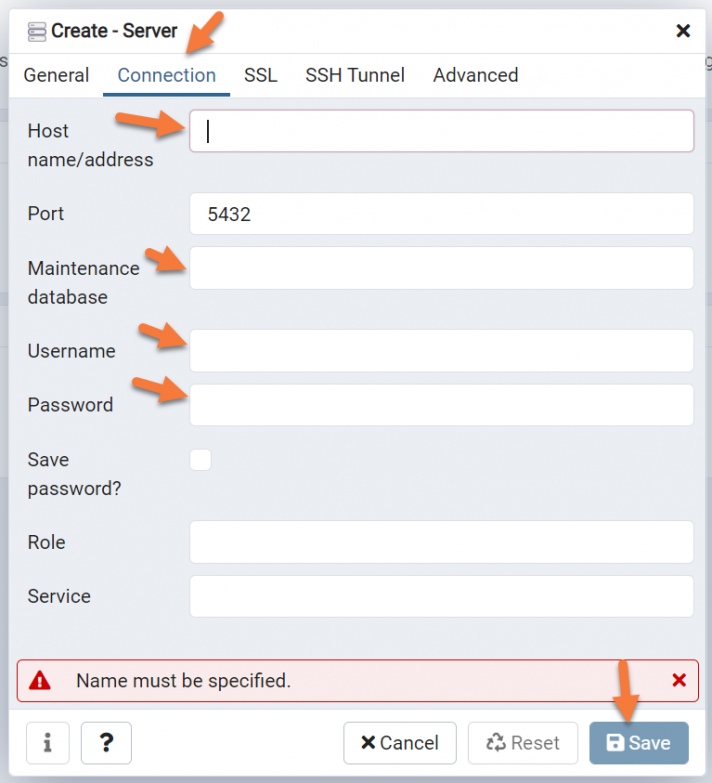
\includegraphics[width=0.9\linewidth]{img/115-712x783.png}
      \label{fig:sub2}
    \end{subfigure}
    \caption{Spajanje na sustav za upravljanje bazom podataka}
    \label{fig:test}
    \end{figure}

    Desnim klikom na upravo povezan poslužitelj, koji se nalazi u lijevoj traci alata, dolazimo do opcije "Create Database". Bazi podataka je potrebno dodijeliti ime i zatim je možemo pohraniti.
    Desnim klikom na novu bazu podataka dolazi se do opcije "Query Tool" koja otvara prozor s mogučnošću unosa nove SQL naredbe. Potrebno je kopirati sadržaj datoteke db.sql koja se nalazi unutar repozitorija te je zatim pokrenuti. Kopirane naredbe će stvoriti sve potrebne tablice, korisnike, uloge...

    \subsection{Backend poslužitelj}

    Prvi korak je izgradnja jar datoteke. Iz direktorija \textit{IzvorniKod/backend} potrebno je pokrenuti naredbu
    \begin{lstlisting}[language=bash]
      mvn package
    \end{lstlisting}
    Ako sve prođe po planu, generiranu jar datoteku koja se nalazi u target direktoriju, potrebno je kopirati na poslužitelj.
    Zatim je na poslužitelju potrebno stvoriti novi servis s putanjom \textit{/etc/systemd/system/dogfriendly-backend.service} i u njega staviti sljedeći kod
    \begin{lstlisting}[language=bash]
        [Unit]
        Description=Spring Boot backend for DogFriendly application
        After=network.target
        StartLimitIntervalSec=0
        
        [Service]
        Type=simple
        Restart=always
        RestartSec=1
        User=root
        ExecStart=/usr/bin/java -jar /home/leon3428/backend/DogFriendly-0.0.1-SNAPSHOT.jar
        
        [Install] 
        WantedBy=multi-user.target
    \end{lstlisting}
    
    Novonastali sevis tada možemo pokrenuti s
    \begin{lstlisting}[language=bash]
        sudo systemctl enable dogfiendly-backend.service
    \end{lstlisting}

    \eject
    \subsection{Frontend poslužitelj}

    Poslužitelj nginx instaliramo s
    \begin{lstlisting}[language=bash]
        sudo apt update
        sudo apt install nginx
    \end{lstlisting}
    Nakon što instalacija završi, potrebno je omogućiti port
    \begin{lstlisting}[language=bash]
        sudo ufw allow 'Nginx HTTP'
    \end{lstlisting}
    Sljedeći korak je konfiguracija bloka za dogfriendly domenu
    \begin{lstlisting}[language=bash]
        sudo mkdir -p /var/www/your_domain/html
        sudo chown -R $USER:$USER /var/www/your_domain/html
        sudo chmod -R 755 /var/www/your_domain
    \end{lstlisting}
    Potrebno je kopirati sljedeću konfiguraciju u datoteku \textit{/etc/nginx/sites-available/your\textunderscore domain}
    \begin{lstlisting}[language=bash]
        server {
                listen 80;
                listen [::]:80;
        
                root /var/www/dog-friendly.me/html;
                index index.html index.htm index.nginx-debian.html;
        
                server_name dog-friendly.me www.dog-friendly.me;
        	access_log  /var/log/nginx/access.log;
        	
        	location / {
            		try_files $uri /index.html;
        	}
        	location /api {  
          		proxy_pass http://localhost:5000;
          		proxy_http_version 1.1;
          		proxy_set_header Upgrade $http_upgrade;
          		proxy_set_header Connection 'upgrade';
          		proxy_set_header Host $host;
          		proxy_cache_bypass $http_upgrade; 
        	}
        }

    \end{lstlisting}
    Konfiguracijsku datoteku omogućimo s
    \begin{lstlisting}[language=bash]
        sudo ln -s /etc/nginx/sites-available/your_domain /etc/nginx/sites-enabled/
    \end{lstlisting}
    Poslužitelj bi sada trebao biti aktivan. Preostaje nam samo izgraditi React aplikaciju što možemo jednostavno napravit s naredbom
    \begin{lstlisting}[language=bash]
        npm run build
    \end{lstlisting}
    pozvanom iz direktorija \textit{IzvorniKod/frontend}.
    Sadržaj build direktorija je sada potrebno kopirati u direktorij \textit{/var/www/your\textunderscore domain/html} na poslužitelju.
    
		\chapter{Zaključak i budući rad}

    Projektni zadatak naše grupe bio je izrada aplikacije DogFriendly, web aplikacije koja bi vlasnicima pasa omogućila lakše pronalaženje željenih i potrebnih lokacija. Također, s obzirom da na aplikaciji postoje i promovirane lokacije vlasnicima obrta bi to služilo kao reklama. \newline

    Sam proces izrade projekta podijeljen je u 2 ciklusa. Prvi ciklus trajao je 8 tjedana. Započeo je s izradom početnog dijela dokumentacije, definiranjem temeljnih zadataka na osnovnoj razini, a potom detaljnijeg proučavanja. Nakon što je u dokumentaciji završena ideja i dogovorena arhitektura započeli smo s programiranjem. S obzirom da se većina tima prvi put susrela s tehnologijama koje smo odabrali koristiti, na početku je uloženo znatno vrijeme u učenje, istraživanje i grupno rješavanje određenih problema. Na kraju prvog ciklusa bio je završen potrebni dio dokumentacije s generičkim funkcionalnostima aplikacije (registracija i prijava), implementiranom kartom i osnovnim prikazom podataka korisnika. \newline

    U drugom ciklusu, u trajanju od 7 tjedana, bilo je potrebno ostvariti ostale funkcionalnosti aplikacije i dovršiti dokumentaciju. Većina backend dijela aplikacije je bila gotova tako da je fokus bio na funkcionalnostima u frontend dijelu i mapbox API-u koji smo koristili za prikaz karte i podataka na karti. \newline

    Na kraju smo uspjeli ostvariti sve funkcionalnosti koje su bile zadane u zadatku. U slučaju da se aplikacija ide učiniti javnom primarno bi se morao pronaći drugi server kako bi se sama aplikacija ubrzala i imala više radne memorije i memorije za spremanje. Također, morao bi se odabrati određeni servis koji bi regulirao spremanje kartičnih podataka obrta i samu naplatu za promociju. \newline

    Na ovom projektu smo svi stekli važna znanja i iskustvo. Naučili smo kako funkcionira timski rad na nekoj aplikaciji i kako se dijeli posao. Vjerujem da će nam stečeno zanje pomoći u daljnjim projektima i olakšati barem početak, koji nam je na ovom projektu bio vrlo velik izazov.

    
    
		\chapter*{Popis literature}

    \begin{enumerate}
        \item Programsko inžinjerstvo, FER, https://www.fer.unizg.hr/predmet/proinz
        \item Astah Community, http://astah.net/editions/uml-new
        \item The Unified Modeling Language, https://www.uml-diagrams.org/
        
    \end{enumerate}
		
		\begingroup
		\renewcommand*\listfigurename{Indeks slika i dijagrama}
		\renewcommand*\listtablename{Indeks tablica}
		\let\clearpage\relax
		\listoffigures
		\vspace{10mm}
		\listoftables
		\endgroup
		\addcontentsline{toc}{chapter}{Indeks slika i dijagrama}
		
		\eject 
		
		\chapter*{Dodatak: Prikaz aktivnosti grupe}

    \section*{Dnevnik sastajanja}
    
    \begin{packed_enum}
        \item sastanak
        
        \item[] \begin{packed_item}
				\item Datum: 20.10.2022.
				\item Prisustvovali: Svi
				\item Teme sastanka:
				\begin{packed_item}
					\item  diskutiranje teme projekta
					\item  početni prijedlozi za način rada
				\end{packed_item}
			\end{packed_item}
			
		\item sastanak
        
        \item[] \begin{packed_item}
				\item Datum: 25.10.2022.
				\item Prisustvovali: Svi
				\item Teme sastanka:
				\begin{packed_item}
					\item  dogovoren način rada i arhitektura
					\item  podijeljeni zadatci za razradu dokumentacije
				\end{packed_item}
			\end{packed_item}
			
		\item sastanak
        
        \item[] \begin{packed_item}
				\item Datum: 3.11.2022.
				\item Prisustvovali: Svi
				\item Teme sastanka:
				\begin{packed_item}
					\item  dogovoren sadržaj baze podataka
					\item  napravljene izmjene u dokumentaciji (UC)
				\end{packed_item}
			\end{packed_item}

            \item sastanak
        
        \item[] \begin{packed_item}
				\item Datum: 16.11.2022.
				\item Prisustvovali: Svi
				\item Teme sastanka:
				\begin{packed_item}
					\item  završna revizija dokumentacije
					\item  pregled i testiranje aplikacije
                        \item  priprema za demonstraciju generičke funkcionalnosti
				\end{packed_item}
			\end{packed_item}
            \eject
            \item sastanak
        
        \item[] \begin{packed_item}
				\item Datum: 06.12.2022.
				\item Prisustvovali: Svi
				\item Teme sastanka:
				\begin{packed_item}
					\item  raspisivanje ostalih funkcionalnosti
					\item  podjela zadataka potrebnih za prezentiranje alfa inačice
				\end{packed_item}
			\end{packed_item}

            \item sastanak
        
        \item[] \begin{packed_item}
				\item Datum: 21.12.2022.
				\item Prisustvovali: Svi
				\item Teme sastanka:
				\begin{packed_item}
					\item  prezentiranje alfa inačice
					\item  definiranje konačnog izgleda i funkcija
				\end{packed_item}
			\end{packed_item}

            \item sastanak
        
        \item[] \begin{packed_item}
				\item Datum: 05.01.2023.
				\item Prisustvovali: Svi
				\item Teme sastanka:
				\begin{packed_item}
					\item  podjela zadataka za dokumentaciju
					\item  dogovor oko deploy-a i testiranja
				\end{packed_item}
			\end{packed_item}
   
    \end{packed_enum}
    \eject

	\begin{longtblr}[
		label=none,
		]{
			vlines,hlines,
			width = \textwidth,
			colspec={X[7, l]X[1, c]X[1, c]X[1, c]X[1, c]X[1, c]X[1, c]X[1, c]}, 
			vline{1} = {1}{text=\clap{}},
			hline{1} = {1}{text=\clap{}},
			rowhead = 1,
		} 
		\multicolumn{1}{c|}{} & \multicolumn{1}{c|}{\rotatebox{90}{\textbf{Leon Stjepan Uroić}}} & \multicolumn{1}{c|}{\rotatebox{90}{\textbf{Luka Marković }}} &	\multicolumn{1}{c|}{\rotatebox{90}{\textbf{Filip Jakovina }}} & \multicolumn{1}{c|}{\rotatebox{90}{\textbf{Mario Hošnjak }}} &	\multicolumn{1}{c|}{\rotatebox{90}{\textbf{David Winkler }}} & \multicolumn{1}{c|}{\rotatebox{90}{\textbf{Nela Štubelj }}} &	\multicolumn{1}{c|}{\rotatebox{90}{\textbf{Zoa Horvat }}} \\  
		Upravljanje projektom 		& 2 & 0 & 0 & 0 & 0 & 0 & 0\\ 
		Opis projektnog zadatka 	& 0 & 2 & 4 & 0 & 0 & 0 & 0\\ 
		
		Funkcionalni zahtjevi       & 0 & 0 & 0 & 0 & 0 & 3 & 0 \\ 
		Opis pojedinih obrazaca 	& 0 & 0 & 0 & 3 & 0 & 0 & 3 \\ 
		Dijagram obrazaca 			& 0 & 0 & 0 & 1 & 0 & 0 & 1 \\ 
		Sekvencijski dijagrami 		& 0 & 0 & 0 & 3 & 0 & 0 & 0 \\ 
		Opis ostalih zahtjeva 		& 0 & 0 & 0 & 1 & 0 & 0 & 0 \\ 
		
		Arhitektura i dizajn sustava	 & 0 & 0 & 0 & 0 & 4 & 0 & 0 \\ 
		Baza podataka				& 5 & 0 & 0 & 0 & 0 & 0 & 0  \\ 
		Dijagram razreda 			& 1 & 0 & 3 & 0 & 0 & 0 & 0  \\ 
		Dijagram stanja				& 0 & 2 & 0 & 0 & 0 & 0 & 0 \\ 
		Dijagram aktivnosti 		& 0 & 0 & 0 & 0 & 0 & 2 & 0 \\ 
		Dijagram komponenti			& 0 & 2 & 0 & 0 & 0 & 0 & 0 \\ 
		Korištene tehnologije i alati 		& 0 & 1 & 0 & 0 & 0 & 0 & 0 \\ 
		Ispitivanje programskog rješenja 	& 0 & 4 & 2 & 4 & 0 & 0 & 0 \\ 
		Dijagram razmještaja			& 0 & 0 & 1 & 0 & 0 & 0 & 0 \\ 
		Upute za puštanje u pogon 		& 3 & 0 & 0 & 0 & 0 & 0 & 0 \\  
		Dnevnik sastajanja 			& 0 & 1 & 0 & 0 & 0 & 0 & 0 \\ 
		Zaključak i budući rad 		& 0 & 1 & 0 & 0 & 0 & 0 & 0 \\  
		Popis literature 			& 0 & 0.5 & 0 & 0 & 0 & 0 & 0 \\  
		&  &  &  &  &  &  &  \\ \hline
            &  &  &  &  &  &  &  \\ \hline
		\textit{frontend} 			& 20 & 40 & 3 & 40 & 30 & 12 & 35 \\ 
		\textit{backend} 				& 40 & 0 & 50 & 2 & 0 & 0 & 0 \\  
		\textit{izrada baze podataka} 		 	& 4 & 0 & 0 & 0 & 0 & 0 & 0\\  
		&  &  &  &  &  &  &\\ 
	\end{longtblr}

\section*{Dijagrami pregleda promjena}
    \begin{figure}[H]
        \centering
        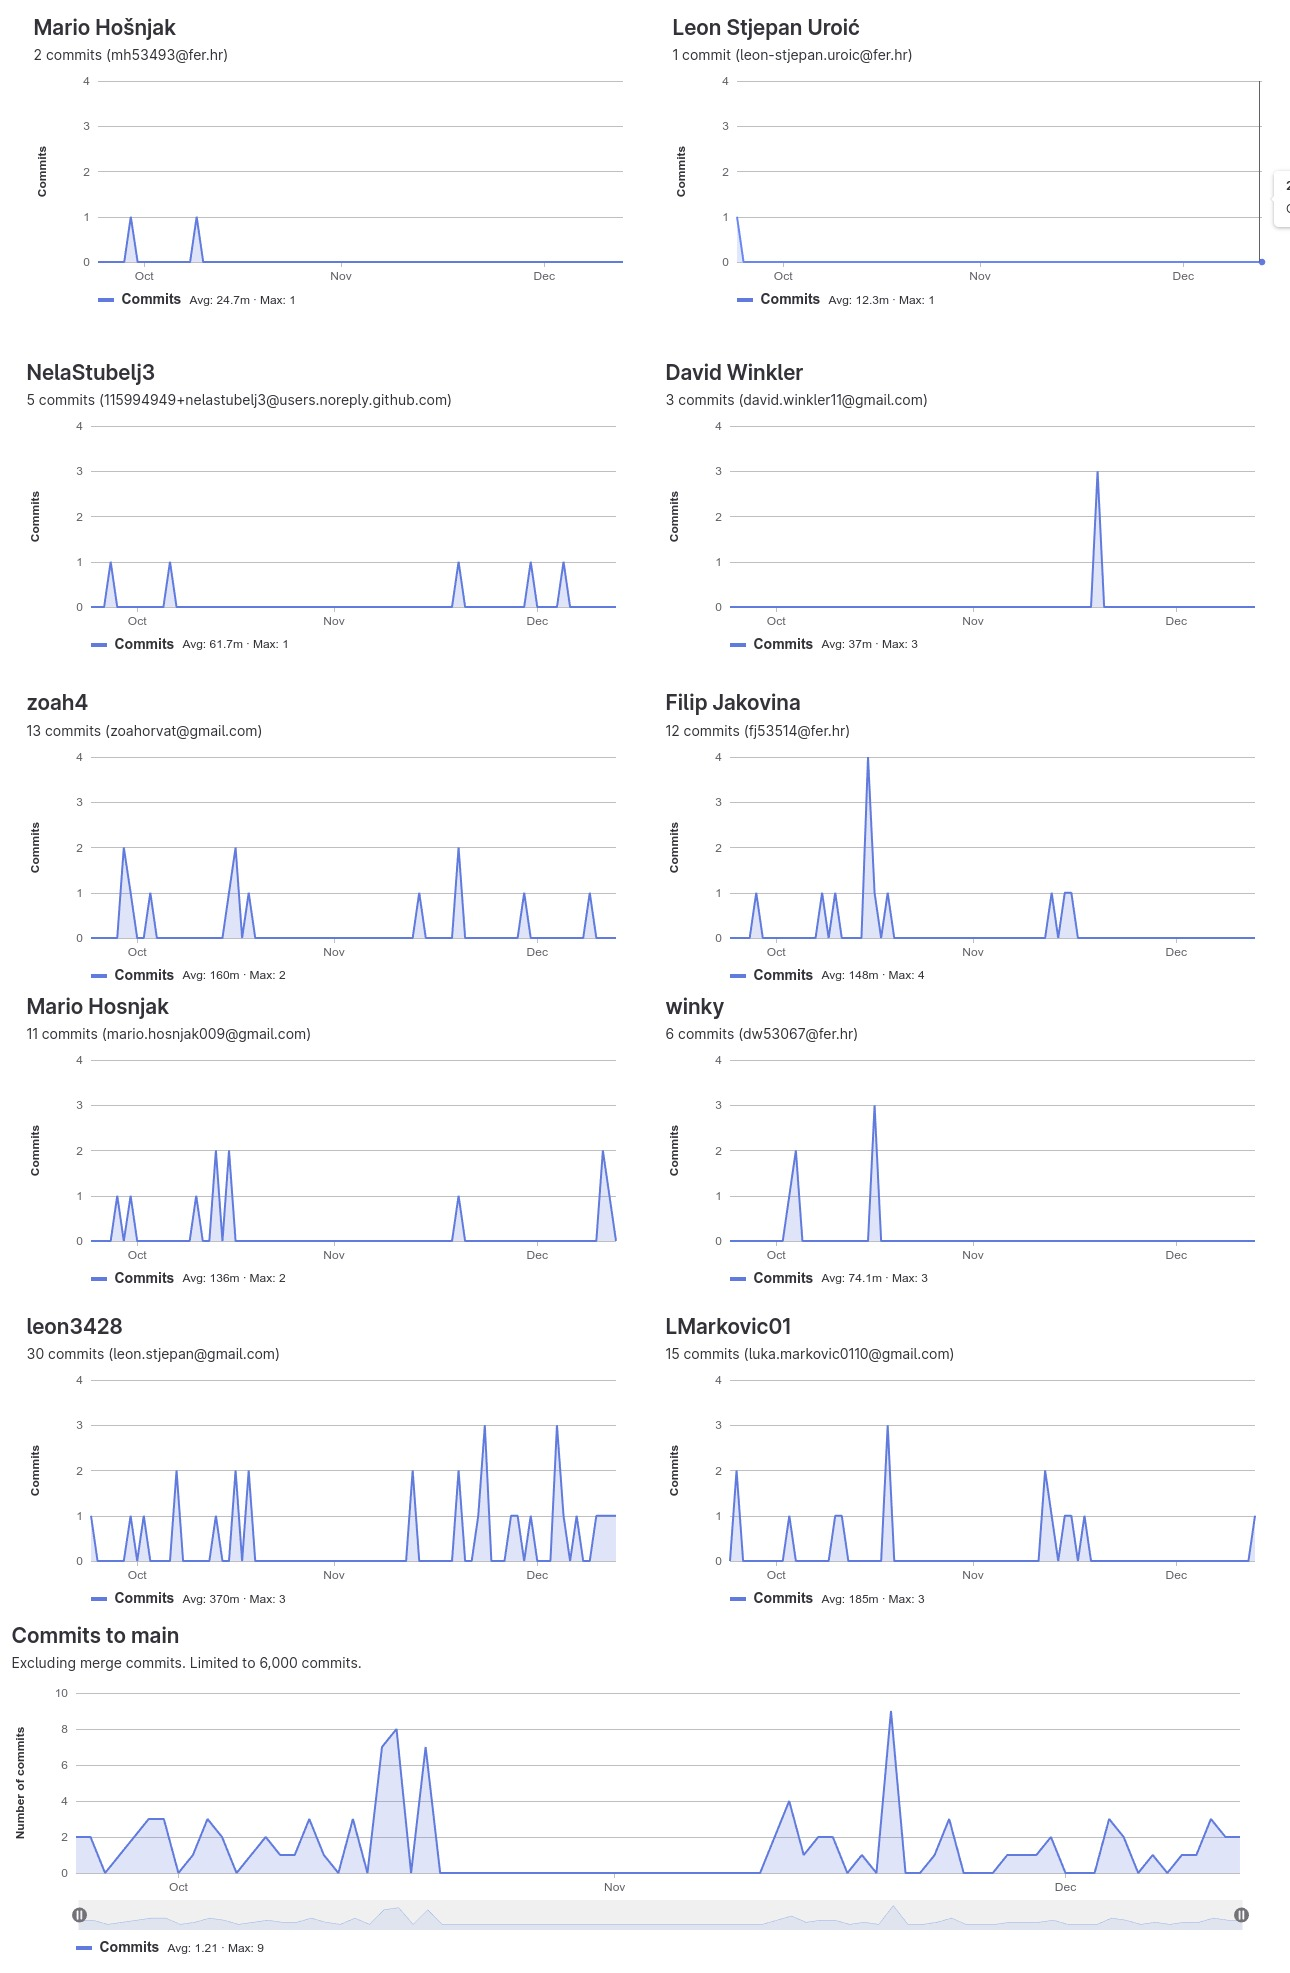
\includegraphics[scale=0.3]{Dokumentacija/img/promjene.jpg}
        \caption{Dijagram pregleda promjena}
    \end{figure}
		
	\end{document} %naredbe i tekst nakon ove naredbe ne ulaze u izgrađen dokument 